\documentclass[letterpaper,12pt]{article}
\usepackage{tabularx} % extra features for tabular environment
\usepackage{amsmath}  % improve math presentation
\usepackage{graphicx} % takes care of graphic including machinery
\usepackage[margin=1in,letterpaper]{geometry} % decreases margins
\usepackage{cite} % takes care of citations
\usepackage{longtable}
\usepackage{booktabs}
\usepackage{fixmath}
\usepackage{amsmath}
\usepackage{amssymb}
\newcommand{\R}{\mathbb{R}}
\usepackage[final]{hyperref} % adds hyper links inside the generated pdf file
\hypersetup{
	colorlinks=true,       % false: boxed links; true: colored links
	linkcolor=blue,        % color of internal links
	citecolor=blue,        % color of links to bibliography
	filecolor=magenta,     % color of file links
	urlcolor=blue         
}
\usepackage{gensymb}
\usepackage{blindtext}
%++++++++++++++++++++++++++++++++++++++++


\begin{document}

\title{Robotics and Deep Learning}
\author{Michele Antonazzi}
\date{\today}
\maketitle

\begin{abstract}
This work is an overview concerning robotics and the machine learning applications can have on it, with a particular focus on deep learning.  
\end{abstract}

\section{Introduction}\label{header-n3}

In the last few years, advances in technologies and research have had a
great impact on the development of robotics. The robots are employed
every day in a large variety of contexts. They substitute humans in
those activities that can be performed more quickly and precisely. An
example is manufacturing when the production process is automatized
using artificial agents to improve productivity and reduce costs. In
this case, the robots are fixed manipulators with a limited range of
motions, that depends on where it is bolted down. This characteristic
strongly limits the agent's possibilities. Generally, a fixed robot is
programmed to perform a single precise task and it operates in a
controlled environment. This means that the algorithm foresees every
possible situation and often it is coded as a state machine. In
contrast, mobile robots would be able to travel within the environment
in which they operate, applying their talents wherever it is most
effective. Thank mobility, the robotics applications become almost
limitless. Some of them are healthcare, entertainment, and rescue.
Mobile robots are also employed in those tasks that are impossible or
too dangerous for humans, as the exploration of hostile environments: a
building on fire, the seabeds, or the surface of another planet. These
robots can be controlled by humans or can be autonomous. The firsts are
controlled through remote controls while the seconds perceive the
environment and move autonomously according to their task, without human
intervention. The main problem that a mobile robot has to solve is how
to move inside the environment. The first aspect is the \emph{motion
	control}. Each robot has a different locomotion system, specific for the
characteristics of the environment in which it moves. Given its
low-level complexity, the motion actions are performed by a specific
software component. To perform the motion control task is necessary to
use the kinematics: the study of how the robot's mechanical systems
behave. To define the kinematics of a robot, it is necessary to define a
geometrical model (specific for the mechanical characteristics of the
locomotion system) that allows expression of robot motion in a global
reference frame and in the robot's local reference frame. Using this
notation, it is possible to define the robot's kinematics model that
describes the movements and their constraints as a function. Through
kinematics, it is resolved the significant challenge of \emph{position
	estimation}. The next step is the \emph{perception}. An autonomous
system has to acquire knowledge about the environment. This is done by
taking measurements using various sensors and then extracting
information from those measurements. With this information, a mobile
robot can determine its position in the environment. This activity is
called \emph{localization}. The last step for an autonomous mobile agent
is \emph{navigation}. Given partial knowledge about its environment and
a goal position or a series of positions, navigation is the ability of
the robot to act based on its knowledge and sensor values to reach its
goal positions as efficiently and as reliably as possible. There are two
main sub-task of navigation: \emph{path planning} and \emph{obstacle
	avoidance}. The first involves identifying a trajectory that will cause
the robot to reach the goal location when executed. The second consists
of modulating the trajectory of the robot in order to avoid collisions.
Using the techniques explained before, an autonomous mobile robot is
able to robustly navigate inside an environment to perform its tasks.
However, a mobile robot operates in a highly non-deterministic context
and the conventional algorithms often are not suitable or not robust
enough. In the real world, in fact, there are a lot of different tasks
that are too complicated to be modeled by a conventional algorithm. Some
problems indeed may have a wide amount of data difficult to analyze. In
this case, build a specific algorithm means to understand the complex
patterns and the hidden correlations between the data. Instead, other
tasks may be influenced by a lot of external factors that generate a
large quantity of similar but different data. These factors are not easy
to model, especially considered all together, and often they are not a
priori known. This means that an algorithm performs well only in a
controlled environment, that respects specific preconditions. On the
other hand, if it is applied in the real world, the algorithm may
encounter data that it cannot correctly analyze. A particular field of
Computer Science is particularly suitable to solve these situations:
\emph{machine learning} (ML). It represents a family of algorithms that
learn automatically through experience. These algorithms are not
designed for a specific task but they are general purposes so they can
be used to solve each type of task. The principle behind machine
learning is the following: each real phenomenon can be modeled as an
unknown mathematical function which can be approximate by a machine
learning algorithm. In this work, the focus is posed on \emph{deep
	learning} and its application to robotics. Deep learning is based on
artificial neural networks, inspired by the biological neural network
that composed the animal brains. In the following sections are resumed
some papers that apply deep learning to robotics. Each of them specifies
the article title, the name of the journal where it has been published,
and the publication year. For each article is summarized the approach
proposed, the innovation with respect to the literature and the
achievements.
\newpage

\section{The limits and potentials of deep learning for
robotics}\label{header-n5}

\emph{THE INTERNATIONAL JOURNAL OF ROBOTICS RESEARCH 2018, Vol. 37(4--5)
405--420} {[}1{]}

\subsection{Introduction}\label{header-n7}

A robot is an inherently active agent that interacts with the real world
and often operates in uncontrolled or detrimental conditions. Mistakes
can lead to potentially catastrophic results, like put human lives at
risk, e.g. if the robot is a driverless car. The application of deep
learning in robotics, therefore, motivates research questions that
differ from those typically addressed in other domains. How much trust
can we put in the predictions of a deep learning system when
misclassifications can have catastrophic consequences? How can we
estimate the uncertainty in a deep network's predictions and how can we
fuse these predictions with prior knowledge and other sensors in a
probabilistic framework? How can we generate enough high-quality
training data? We can obtain these data in real-world scenarios or we
can obtain them using data augmentation through simulation? Is there a
fundamental difference between model-driven and data-driven
problem-solving? This paper explores some of the challenges, limits, and
potentials for deep learning in robotics.

\subsection{Challenges for deep learning in robotic
vision}\label{header-n9}

\begin{figure}[h!]
	\centering
	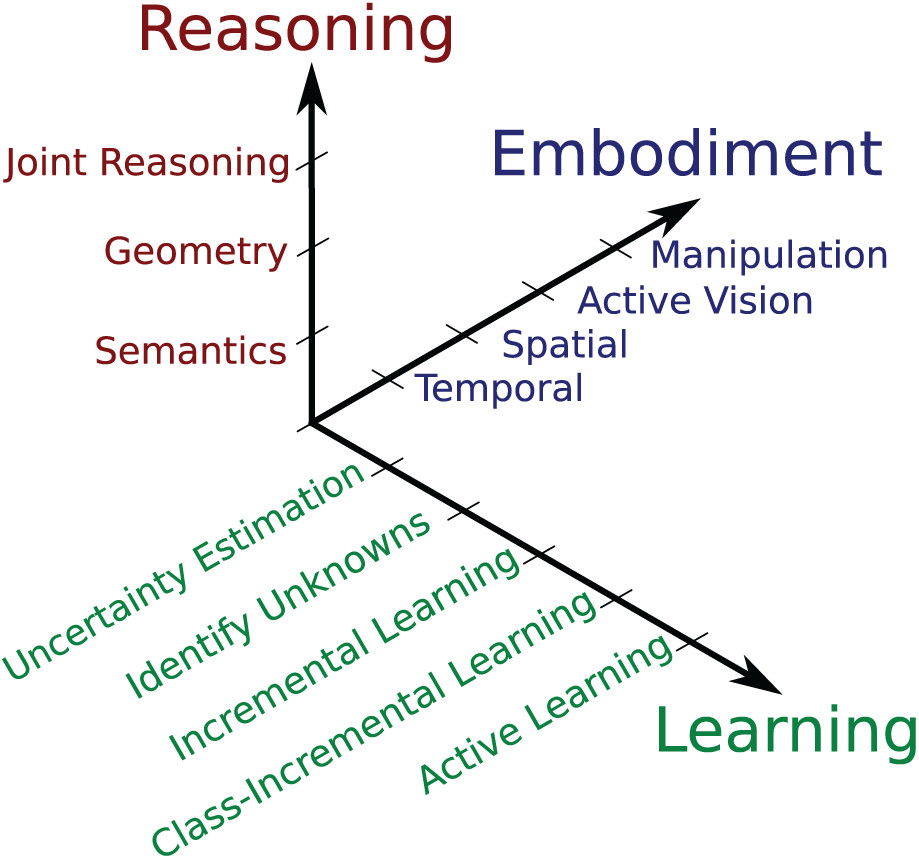
\includegraphics[width=0.5\linewidth]{images/roboticvision.jpeg}
	\caption{Current challenges for deep learning in robotic vision}
\end{figure}

\emph{Robotic vision} differs from \emph{computer vision} in several
aspects. In particular, the latter is a part of the first. A robot is an
active agent that perceives the world with its different sensors, builds
a coherent model of the world, and updates this model over time, but
ultimately a robot has to make decisions, plan actions, and execute
these actions to fulfill a useful task. In fact, for robotic vision,
perception is only one part of a more complex system. In a simplified
view, whereas computer vision takes images and translates them into
information, robotic vision translates images into actions. This
fundamental difference between robotic vision and computer vision
motivates a number of research challenges along three conceptually
orthogonal axes: \emph{learning}, \emph{embodiment}, and
\emph{reasoning}. We position individual challenges along these axes
according to their increasing complexity, and their dependencies.



\subsubsection{Learning challenges}\label{header-n12}

Along this axis, we position challenges that are specific for (deep)
machine learning in a robotic vision context.

\paragraph{Uncertainty estimation}
It is important that deep learning systems can reliably estimate the
uncertainty in their predictions. The robot has to treat a neural
network in the same way as other sensors, also using Bayesian techniques
to fuse the network's predictions with prior knowledge to accumulate
information over time. Typically a deep learning model returns scores
that are not calibrated probabilities so not useable in a Bayesian
sensor fusion framework. 
\paragraph{Identify unknowns}

A common assumption in deep learning is that trained models will be
deployed under \emph{closed-set} conditions. However, robots often have
to operate in ever-changing, uncontrolled real-world environments, and
they will inevitably encounter data not covered by the training data. In
these \emph{open-set} conditions, it is crucial to identify unknowns
with high confidence.
\paragraph{Incremental learning}

A robotic vision system should be able to learn from new training
samples of known classes during deployment, upgrading its internal
representations accordingly.

\paragraph{Class-incremental learning}

A robot, therefore, needs the capability to extend its knowledge and
efficiently learn new classes of interest without forgetting the
previously learned ones. Current techniques for class-incremental
learning still rely on supervision in the sense that the user has to
specifically tell the system which samples are new data.

\paragraph{Active learning}

A robot should be able to select the most informative samples for
incremental learning techniques on its own. In order to minimize the
interaction with the humans, the robotic system can also comprise
retrieving annotations from other sources such as the web.

\newpage
\subsubsection{Embodiment challenges}\label{header-n24}

\paragraph{Temporal embodiment}

A robotic vision system perceives a stream of consecutive and therefore
strongly correlated images. The potential of temporal embodiment to
improve the quality of the perception process for object detection or
semantic segmentation is currently rarely utilized. A robotic vision
system that uses its temporal embodiment can, for example, accumulate
evidence over time or exploit small viewpoint variation. A challenging
aspect of the temporal embodiment is that the appearance of scenes
changes over time. An environment can comprise dynamic objects which
move inside it. Besides, an environment can also change its appearance
according to different lighting conditions (day/night), structural
changes in objects (summer/winter).

\paragraph{Spatial embodiment}

The camera of a robotic system is spatially embodied and it will observe
the scene according to the robot's movements. This fact poses both
challenges and opportunities to a robotic vision system: it can help to
disambiguate its semantic properties, improve depth perception, or
segregate an object from other objects or the background in cluttered
scenes. On the other hand, occlusions can alter or changes the visual
perception.

\paragraph{Active vision}

One of the biggest advantages of a robot is the potential to control the
camera, move it, and change its viewpoint independently from the robot's
movements. In this way, a dynamic robotic vision system can improve its
perception confidence, resolve ambiguities, and mitigate the effect of
occlusions or reflections.

\paragraph{Manipulation for perception}

As an extension of active vision, a robotic system could manipulate the
scene to improve its perception. For example, a robot could move
occluding objects or move an object to see its occluded faces.

\subsubsection{Reasoning challenges}\label{header-n33}

Von Helmholtz (1867) formulated the idea that humans use unconscious
reasoning when processing visual information, in order to inference
concepts or make conclusions. The following searches investigate these
unconscious mechanisms and reformulated them in a Bayesian inference
framework.

\paragraph{Reasoning about object and scene semantics}

The world around us contains many semantic regularities that humans use
to aid their perception: objects tend to appear more often in a certain
context, some objects tend to appear in groups, some objects rarely
appear together in a scene, and so on. If these semantic regularities
can be used by a vision system as prior knowledge, we can expect an
improved and more robust vision framework.

\paragraph{Reasoning about object and scene geometry}

Many applications in robotics require knowledge about the geometry of
individual objects, or the scene as a whole. Estimating the 3D structure
of scenes or objects from multiple views without having depth
information is a widely researched topic. A robot, differently from a
classical approach, has to perform this task in cluttered scenes, where
the objects are not clearly separated. A robot needs the ability to
express uncertainty in the inferred object shape and it should be able
to exploits its embodiment to move the camera to collect new and more
useful information. Inference over the geometry of the whole scene is
related also to object-based simultaneous localization and mapping
(SLAM).

\paragraph{Joint reasoning about semantics and geometry}

The final reasoning challenge for a robotic vision system, therefore, is
the ability to reason jointly about the semantics and the geometry of a
scene. Semantics and geometry can help each other: a tightly coupled
inference approach can be advantageous compared to two systems that work
separately.

\subsection{The evaluation method for deep learning models applied to
robotics}\label{header-n41}

Normally the good deep learning performance is not reached when the
models are used in real environments. The evaluation method used in
computer vision fails when applied in robotics: a robot has to interact
with a dynamic environment and not with a simple set of images
downloaded from the Internet. When a statistic report indicates that a
dataset has been solved, it does not necessarily mean that the problem
itself has been solved. The available datasets often are not able to
able to correctly evaluate the performance of a robotic deep learning
model. One of the reasons is the datasets' inability to give to the
model information about the unknowns aspect of real environments. In
particular, \emph{Open set recognition} refers to scenarios where
incomplete knowledge of the world is present at training time. This
implies that unknown classes can be submitted to the model during its
operation. What is needed is a new class of machine learning algorithms
that minimize the risk of the unknown. To do this, updated evaluation
protocols are also needed. These protocols have to incorporate data that
is both know and unknown to a model. Another important aspect is the
systematic study of the performance of a recognition model across an
exhaustive range of object appearances. To better understand this
mechanisms, inner in the humans' visual system, psychophysics discipline
can be used. Psychophysics investigates the relationship between
physical stimuli and the sensations and perceptions they produce. This
concept can be translated into the field of deep learning: we would like
to know under what conditions a machine learning model is able to
operate successfully, as well as where it begins to fail. But how
exactly can Psychophysics be applied to deep models? One possibility is
through a computational pipeline that is able to perturb the data at a
massive scale (e.g. millions of images per image transformation being
studied) and submit them to a model, studying its performance through
the item--response curve. The key to interpreting the results is the
ability to identify the model's preferred view. The preferred view
concept derives from vision science, which has established that humans
possess an internalized canonical view (the visual appearance that is
easiest to recognize) for individual object classes. Similarly,
recognition models have one or more preferred views of an object class,
each of which leads to a maximum (or minimum) score output. The
psychophysics progresses support a growing trend in robotics and
computer vision: simulation using rendered graphics. The models'
performance can be assessed by comparing the respective item--response
curves. Importantly, this technique can find potential gaps not only
between different models but also between human and model behavior.
Human performance vastly exceeds model performance even in cases where a
problem has been assumed to be solved, especially comparing the
item-response curves.

\subsection{The role of simulation for pixel-to-action
robotics}\label{header-n43}

\emph{Deep reinforcement learning} is a new learning paradigm that is
capable of learning end-to-end robotic control tasks, but its results
have been demonstrated primarily in simulation, rather than on real
robot platforms. Demonstrating learning capabilities on real robots
remains a significant challenge: the long, data-hungry training paradigm
of pixel-based deep robotic learning methods are too computationally
hard to be executed by a robotic platform. On the other hand, in
simulation, the training time can be greatly reduced by using dedicated
hardware and parallelism paradigms. Another important difference that
often separates a simulated task and its real-world analog concerns raw
pixel inputs. One solution is to use transfer learning methods, but
there exist fewer approaches for transfer from simulation to reality for
robot domains. Another one consists of augmenting the target
domain data with data from the source domain. Another approach is to use
a ``confusion" loss that forces the model to ignore data variations that
separate the two domains. A more recent simulation-to-real solution
relies on the \emph{progressive network} architecture, which enables
transfer learning through lateral connections that connect each layer of
previously learned deep networks to new networks to model the gap
between the two domains. 
\begin{figure}[h!]
	\centering
	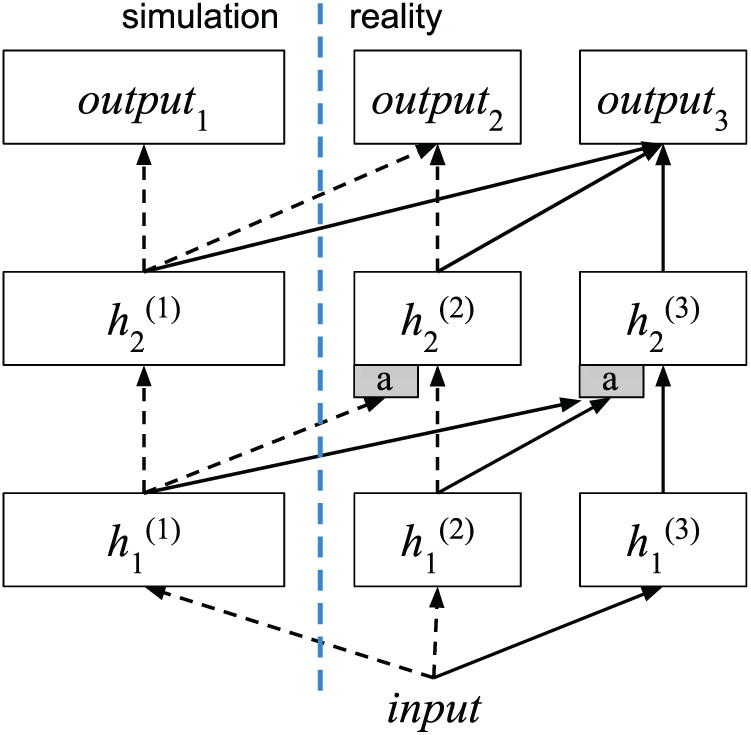
\includegraphics[width=0.5\linewidth]{images/progressivenets.jpeg}
	\caption{Detailed schematic of progressive recurrent network architecture}
\end{figure}

The progressive networks advantages for
simulation-to-real transfer are the following:

\begin{itemize}
\item
  the features learned for one task may be transferred to many new
  tasks;
\item
  the columns may be heterogeneous, which may be important for solving
  different tasks, including different input modalities, or simply to
  improve learning speed when transferring to the real robot;
\item
  progressive nets add new capacity, including new input connections,
  when transferring to new tasks. This is advantageous for bridging the
  reality gap, to accommodate dissimilar inputs between simulation and
  real sensors.
\end{itemize}



\subsection{Deep learning and physics-based models}\label{header-n53}

The predominant approach to perception, planning, and control in
robotics is to use approximate models of the physics underlying a robot,
its sensors, and its interactions with the environment. These models
require that their parameters are known with sufficient accuracy and can
be tracked over time. This requirement poses overly challenging demands
on system identification and perception, resulting in brittle systems.
On the other hand, humans operate under intuitive rather than exact
physical models. For this reason, they are capable of robustly
performing a wide variety of tasks. Also, deep learning is moving in
this direction: a lot of approaches forgot the use of explicit physics
models, learning predictive models, and controls from raw experiences.
Let's now confront the model-based and deeply learned approaches.
Model-based approaches have wide applicability since the physics
underlying them are universal. However, at the same time, the parameters
of these models are difficult to estimate from perception. Deep
learning, on the other hand, enables highly robust performance when
trained on sufficiently large data sets but it does not have the general
applicability of physics-based reasoning. Model-based approaches are
significantly more data-efficient, related to their smaller number of
parameters but the basin of convergence can be rather small. In
contrast, deep learned solutions are often very fast and can have very
large basins of convergence. However, they do not perform well if
applied in a regime outside the training data. The following table
resumes the principles just reported.

\begin{longtable}[]{@{}lll@{}}
\toprule
& \textbf{Model-based} & \textbf{Deep learning}\tabularnewline
\midrule
\endhead
\emph{Presentation} & Explicit: based on or inspired by physics &
Implicit\tabularnewline
\emph{Generality} & Broadly applicable (physics are universal) & Only in
trained regime\tabularnewline
\emph{Robustness} & Small basin of convergence  & Large basin of convergence
\tabularnewline
Data efficiency & Very high &
Training requires a lot of data \tabularnewline
Computational efficiency & Good in local regime & Highly efficient once
trained\tabularnewline
\bottomrule
\caption{Models versus deep learning}
\end{longtable}

\newpage
\subsection{Towards an automation of informatics}\label{header-n80}

Deep learning will change the foundations of computer science. The
successes of deep learning in various domains changing the algorithm
design paradigm. While designing a specific algorithm requires a lot of
experience and knowledge about the problem domain, machine learning
techniques allow us to solve even a difficult task with little to no
knowledge of the problem domain.

\paragraph{Programming versus data}

The programming paradigm is changing rapidly with the evolution of
machine learning. In traditional computer science, human experts program
problem-specific algorithms that require no additional data to solve a
particular problem instance. On the other hand, a generic learning
approach needs a large amount of data to find a computational solution
automatically. The act of \emph{programming} is replaced by
\emph{training} on the other end. The concept of the program is turned
into the learning weights of the network. The programming language (the
language in which a solution is coded), is replaced by network
architecture, loss function, training procedure, and data.

\paragraph{Does understand imply a precise approach?}

Computer programs reflect human understanding: a programmer has to
understand the problem he is solving. If it is using deep learning
techniques, we might say that less knowledge is required. The trend for
a good programmer should be to understand the problem he is facing. To
do this, often it needs to be able to use generic tools, such as deep
learning, to discover problem structure. Furthermore, a programmer
should understand how problems can be divided into parts: those parts
for which we know the structure (and, therefore, can write algorithms
for) and those for which we would like to discover the structure.

\paragraph{Generic tools might help us identify new structures}

As mentioned before, a programmer can use generic tools to acquire the
knowledge needed to solve a problem and code a specific program. It
might be difficult to extract this knowledge from a deep neural network
but that should simply motivate researchers to develop methods for
extracting this knowledge. This procedure is possible, as shown by
recent experiments, but the extracted knowledge is really difficult to
be used to design a specific algorithm. In addition, the neural networks
further complicate this process: they simply memorize the training
parameters, making so hard to extract the problem structure from them.

\paragraph{Complex problems should be solved by decomposition and
re-composition}

In many cases, interesting and complex problems will exhibit complex
structures because they are composed of sub-problems. For many
sub-problems, we already have excellent algorithmic solutions while, for
many others, domain-specific programs are outperformed by deep neural
networks. The re-composition can be achieved with differentiable
versions of existing algorithms that are compatible solutions obtained
with back-propagation

\paragraph{Decomposability of problems}

A problem is called \emph{decomposable} or \emph{near-decomposable} if
there is little complexity in the interactions among its sub-problems
and most of the complexity is handled within those sub-problems. For
example, the brain is not decomposable because the interactions between
its components still contain much of the complexity of the original
problem. Despite decomposition helps to dominate the problem complexity,
this is not true for deep neural networks. In fact for end-to-end models
giving up strict boundaries between sub-problems improves their
solution. The authors suspect that there are optimal factorizations of
problems for a defined task, agent, and environment. Despite this,
factorization may not lead to simple interfaces between sub-problems but
certainly facilitates finding an optimal solution.

\paragraph{Automating programming}

Programming should be easy to automate. If we can successfully apply
generic methods to complex problems, extract an algorithmic knowledge
from the resulting solutions, use the resulting algorithms to solve
sub-problems of the original problem, thereby making that original
problem more easily solvable, and so forth, then we can also imagine an
automated way of deriving computer algorithms from problem-specific
data. A key challenge will be the automatic decomposition or
factorization of the problem into suitably solvable sub-problems. This
view raises some fundamental questions about the differences between
\emph{programs} in programming and \emph{weights} in deep learning.
Programs and weights, in this view, are different instances of the same
thing: there is no qualitative difference between them. It seems
plausible that when parameters are so specific we can call the program,
but the reverse is also true. It is possible that other problems do not
have algorithmic characteristics and can only be solved in a data-driven
way.

\paragraph{Priors to reduce the amount of data}

The process for acquiring the data can be very costly, especially when
these data have to be acquired from interaction with the real world, as
is the case in robotics. It will then become necessary to reduce the
required amount of data by incorporating appropriate priors into
learning. These priors reduce all possible interpretations of data to
only those consistent with the prior.

\subsection{Conclusions}\label{header-n96}

The robotics community had accepted deep learning as a very powerful
tool and begun to utilize and advance it. Despite this, the authors hope
to see more integrated approaches in the future: robots that learn to
utilize their embodiment to reduce the uncertainty in perception,
decision making, and execution. Robots that learn complex multi-stage
tasks. Robots that learn to discover and exploit the rich semantic
regularities and geometric structure of the world. It is necessary to
keep in mind that robotic perception, robotic learning, and robotic
control are tasks that continue to pose severe challenges to the
techniques typically applied.
\newpage

\section{A Machine Learning Approach to Visual Perception of Forest
Trails for Mobile Robots}\label{header-n5}

\emph{IEEE ROBOTICS AND AUTOMATION LETTERS, VOL. 1, NO. 2, JULY 2016} {[}2{]}

\subsection{Introduction}\label{header-n7}

This article studies the problem of perceiving forest or mountain trails
from a single monocular image acquired from the viewpoint of a robot.
Autonomously following a man-made trail is challenging for robotics.
Many robot types, including wheeled, tracked, and legged vehicles, are
capable of locomotion along real-world trails. Moreover, Micro Aerial
Vehicles (MAVs) flying under the tree are a compelling and realistic
option made possible by recent technological advances. One of the
innovations introduced by this article is that the robot used for the
experiments is a quadrotor: a drone with four rotors. In order to follow
a trail, a robot has to perceive where the trail is, then react in order
to stay on the trail. The robot input is a monocular image from a
forward-looking camera. Perceiving real-world trails in these conditions
is an extremely difficult and interesting pattern recognition problem.
Computer Vision and Robotics literature mainly focused on paved road and
forest/desert road perception. The latter is a significantly more
difficult problem: unpaved roads are normally much less structured than
paved ones. Their appearance is very variable and often boundaries are
not well defined. In addition, their surface appearance can change very
frequently, their shape and width are not as constrained, they often
seamlessly blend with the surrounding area. Previous works deal with the
task of perceiving trails as a segmentation problem, aiming to determine
which areas of the input image corresponding to the image of the trail.
To do this, it is necessary to classify the visual features that
characterize a trail. All of these techniques are conceptually similar
to image saliency. A \emph{saliency map} is an image that shows for each
pixel (of the original image) how much such pixel visually ``stands out"
from the rest. This information, which by itself is expected to be very
noisy, is aggregated in order to infer the trail position and direction
in the image. In this work, the authors follow a different approach and
cast the trail perception problem as an image classification task. The
robot estimates the approximate direction of the trail with respect to
the direction of view by adopting a supervised machine learning approach
based on Deep Neural Networks (DNNs). One of the advantages of DNNs for
supervised image classification is generality: in fact, features are
learned directly from data and do not have to be chosen or modeled by
the algorithm developers for the specific problem. Deep learning is used
also for obstacle avoidance. Previous work shows how imitation learning
can be used to steer a quadrotor to avoid trees in an outdoor
environment. The controller is previously trained by manually piloting
the robot for a short time. However, the visual perception task is
harder, requiring a more powerful classifier to be trained with a
significantly larger training dataset obtained offline.

\subsection{Proposed method}\label{header-n9}

\subsubsection{Problem formulation}\label{header-n10}

The robot consists of a MAV with a monocular camera, fixed in front of
it. The drone flies with a height similar to the average height of a
person (approximately 1.7 meters). The input is an image acquired by the
camera. The main goal is to remain on the trail analyzing the image
using a deep learning module. There are considered three different
classes which correspond to three different actions that the robot
should implement in order to remain on the trail:

\begin{itemize}
\item
  \textbf{Turn Left (TL):} if $−90\degree \textless{} \alpha \textless{} −\beta$; the
  trail is heading towards the left part of the image
\item
  \textbf{Go Straight (GS):} if $−\beta \leq  \alpha \textless{} +\beta$; the trail is
  heading straight ahead, at least in the close range
\item
  \textbf{Turn Right (TR):} if $+\beta \leq \alpha \textless{} +90\degree$; the trail is
  heading towards the right part of the image
\end{itemize}

With $\beta$ = 15\degree.

\begin{figure}[h!]
	\centering
	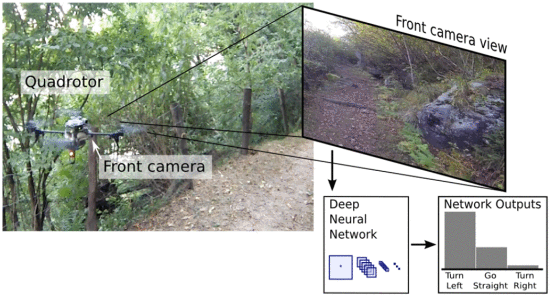
\includegraphics[width=0.8\linewidth]{images/quad.png}
	\caption{The proposed method's overview}
\end{figure}

\subsubsection{Dataset}\label{header-n47}

Recognize a trail is a very hard task and the learning machine needs a
large and well-formed dataset to perform this task effectively. Such a
dataset does not exist and the authors had to create it from scratch. A
hiker was equipped with three head-mounted cameras: one pointing 30◦ to
the left, one pointing straight ahead, and one pointing 30◦ to the
right. The fields of view of the three cameras partially overlap and
cover approximately 180 degrees. The hiker then swiftly walks a long
trail, by taking care of always looking straight along its direction of
motion. The dataset is composed of the images acquired by the three
cameras, labeled as follows: all images acquired by the central camera
are of class GS, those acquired by the right camera are of class TL and
the others (acquired by the left camera) make up the TR class. The
dataset is composed of 8 hours of $1920 \times 1080$ 30fps video acquired using
three GoPro Hero3 Silver cameras and covers approximately 7 kilometers
of hiking trails acquired at altitudes ranging from 300 m to 1200 m,
different times of the day and weather. The dataset has been split into
disjoint training (17,119 frames) and testing (7,355 frames) sets.

\subsubsection{Deep neural network}\label{header-n55}

The authors implement the trail perception module as DNN (deep neural
network), which is a feed-forward network built using successive pairs
of convolutional and max-pooling layers, followed by several fully
connected layers. To improve the network performances, the training set
is augmented by synthesizing left/right mirrored versions of each
training image. Additionally, mild affine distortions ($\pm10\%$
translation, $\pm15^{\circ}$ rotation, $\pm10\%$ scaling) are applied to training
images to further increase the number of samples. The DNN is trained
using backpropagation for 90 epochs, with a learning rate initially set
to 0.005, then scaled by a factor of 0.95 per epoch. The free parameters
(weights) are initialized with random numbers from a uniform
distribution in the range {[}−0.05, 0.05{]} and they are optimized using
stochastic gradient descent. The network has an input layer formed by a
matrix of $3 \times 101 \times 101$ neurons. To fit with the input layer, the images
are first anisotropically resized (with an anti-aliasing technique) to a
size of $101 \times 101$ pixels. The pixels intensity are rescaled to the range
{[}-1, +1{]}. The DNN's output layer has 3 neurons, one for each of the
three classes TL, TR, GS.

\subsubsection{Experimental results}\label{header-n72}

For the three-class classification problem, the absolute accuracy metric
is computed to evaluate the model performances. To have a more robust
performance evaluation, the authors consider a derived two-class
classification problem. The resulting problem consists in determining if
an image is of class GS or not. There are calculated accuracy,
corresponding precision (the proportion of positive classifications that
are actual positives), recall (the proportion of the actual positives
that are identified correctly), and the area under the ROC curve. The
authors compare the DNN performance to three alternatives:

\begin{itemize}
\item
  \textbf{Simple Saliency-based Model:} it is computed a saliency map of
  the input frame, based on the image hue. The saliency map is
  discretized to $16 \times 9$ blocks, and the average saliency for each block
  yields a 144-dimensional feature vector. An SVM model with an RBF
  kernel is learned from the training set to map this feature vector to
  the three-class: TL, GS, and TR.
\item
  \textbf{The method by Santana et al:} this algorithm is explained in
  {[}12{]} and it is applied to the dataset images (50 iterations per
  frame). Its output trail soft segmentation is sampled at each of the
  testing frames.
\item
  \textbf{Two human observers:} each of which is asked to classify 200
  randomly sampled images from the testing set in one of the three
  classes.
\end{itemize}

The obtained results are reported it the following tables.

\begin{longtable}[]{@{}llllll@{}}

\toprule
& \textbf{DNN} & \textbf{Saliency} & \textbf{{[}2{]}} & \textbf{Human1}
& \textbf{Human2}\tabularnewline
\midrule
\endhead
\textbf{Accuracy} & 85.2\% & 52.3\% & 36.5\% & 86.5\% &
82.0\%\tabularnewline
\bottomrule
\caption{Results for the three-class problem}
\end{longtable}

\begin{longtable}[]{@{}llllll@{}}
\toprule
& \textbf{DNN} & \textbf{Saliency} & \textbf{{[}2{]}} & \textbf{Human1}
& \textbf{Human2}\tabularnewline
\midrule
\endhead
\textbf{Accuracy} & 95.0\% & 73.6\% & 57.9\% & 91.0\% &
88.0\%\tabularnewline
\textbf{Precision} & 95.3\% & 60.9\% & 39.8\% & 79.7\% &
84.0\%\tabularnewline
\textbf{Recall} & 88.7\% & 46.6\% & 64.6\% & 95.1\% &
81.6\%\tabularnewline
\textbf{AUC} & 98.7\% & 75.9\% & - & - & -\tabularnewline
\bottomrule
\caption{Results for the two-class problem}
\end{longtable}

\subsubsection{Conclusion}\label{header-n191}

The model has good performance, even when compared to those of humans.
However, problems arise when applying this model in the real world. The
authors implemented this model in a real drone, with a camera that
captures frames with a resolution of $752 \times 480$ pixels. The main problem
is the much lower image quality acquired by the quadrotors' cameras as
compared to the GoPro's images in the training dataset. This yielded a
lower performance of the classifier compared to the testing dataset.
This was especially apparent in situations with strong sky-ground
contrast. Another problem is related to the trail width: the robot is
often unable to negotiate trails if there is not enough free space
beside the trail centerline. Despite this, on wide trails with even
lighting conditions, the robot was able to successfully follow the trail
for a few hundreds of meters.
\newpage

\section{A Hybrid Compact Neural Architecture for Visual Place
Recognition}

\emph{IEEE ROBOTICS AND AUTOMATION LETTERS, VOL. 5, NO. 2, APRIL 2020}
{[}4{]}

\subsection{Introduction}\label{header-n182}

Performing visual place recognition (VPR) reliably is a challenge for
any robotic system or autonomous vehicle operating over long periods in
real-world environments. Convolutional neural networks (CNN) have been
applied to the field of VPR with great success, typically using
dedicated hardware: the GPUs. However, classical CNNs neglect any
temporal information between consecutive images. However, sequence-based
algorithms, such as SeqSLAM, matching two or more sequences of images to
perform VPR. Two main deep learning models can be used to capture
sequence patterns: \emph{computer-science-oriented} and
\emph{neuroscience-oriented} models. In recent researches, recurrent
neural networks (RNN) are used to reproduce the multi-scale spatial
representation of an environment. While the results are promising, these
computer-science-oriented systems are tested only in small synthetic
environments, and the integration with neuroscience-oriented recurrent
models such as continuous attractor neural networks (CANN) is not well
explored. An attractor network is a network of nodes (i.e. neurons),
often recurrently connected, whose time dynamics settle to a stable
pattern. A pattern can be stationary, time-varying (i.e. cyclic), or
chaotic. The particular pattern which network settles to is called its
\emph{attractor}. In neuroscience theory, different kinds of attractor
neural networks have been associated with different functions, such as
memory, motor behavior, and classification. More in detail, a continuous
attractor network is a special type of attractor network, which models a
non-linear dynamical system. A dynamical system consists of a
\emph{state place}, which its coordinates describe the state at any
instance and a \emph{dynamical role} that specifies the immediate future
of all state variables. For example, the state of a pendulum is its
angle and angular velocity, and the evolution rule is Newton's equation
\emph{F}=\emph{m\^{}a}. An \emph{attractor} can be discrete (a discrete
set of points) or continuous (a continuous object embedded in the state
space).

\begin{figure}[h!]
\centering

\includegraphics[width=0.5\linewidth]{images/continuousattractor.jpg}
\caption{A system (the yellow ball) with a continuous attractor (the blue surface)}
\end{figure}

In this work, the authors propose a hybrid neural network that
incorporates both computer-science- and neuroscience-oriented models to
perform the VPR task. Their approach comprises two key components:
FlyNet, a compact neural network, and a 1-d CANN as a temporal model
that encodes sequences of images to perform appearance-invariant VPR
using real data. The resulting FlyNet+CANN model achieves competitive
AUC results, but with far fewer parameters, minimal training time and
smaller computational footprint than conventional deep learning and
algorithmic-based approaches.

\begin{figure}[h!]
\centering
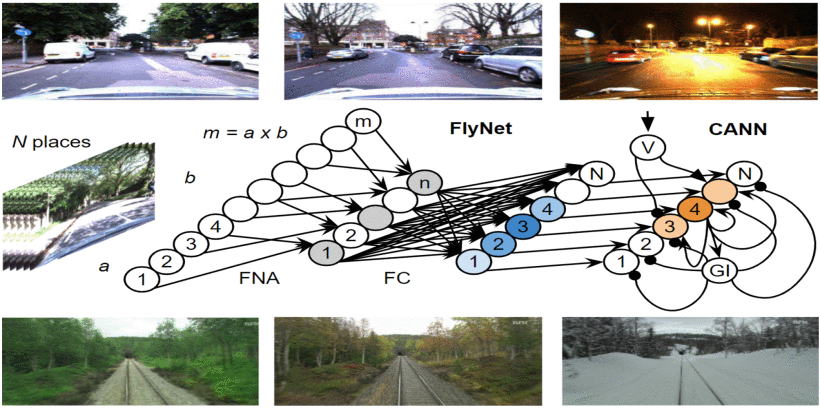
\includegraphics[width=0.8\linewidth]{images/flynetcann.png}
\caption{FlyNet+CANN hybrid neural architecture}
\end{figure}

\subsection{Previous work}\label{header-n187}

To design deep-learning-based models for VPR it is necessary to explore
how this activity is performed by mammalians' brains and take
inspiration from it. RatSLAM is an example, this method performs visual
SLAM implementing the mechanisms using by rodents' brain. Other models
perform VPR following the insect brains, like ants, bees, and flies,
that exhibits the great capacity to navigate. Place recognition in
insects is, however, most likely mediated by processing within the
\emph{mushroom bodies} (MB), a pair of structures involved in
classification, learning, and recognition of both olfactory and visual
information. Their structure has been similar to a multi-layer
perceptron (MLP) network, which receives massive input signals from
sensory lobes. These impressive capabilities, achieved with relatively
small brains, make them attractive models for roboticists. For FlyNet,
we take inspiration from algorithmic insights found in the fruit fly
olfactory neural circuit. The authors investigate how it can be
integrated with recurrent-based networks for the VPR task. Classical CNN
models for image recognition have good performance but they have also
undesirable characteristics. In fact, these networks are difficult to
implement in a real robot, due to their size and complexity. In
contrast, the authors propose the usage of compact neural models such as
FlyNet to alleviate these requirements. To access and exploit the power
of temporal information in many applications, researchers have developed
a range of RNN. Another approach, implementing by RatSLAM, uses
incorporated multi-dimensional CANN models with pre-assigned weights and
structure. There exist other non-neural techniques, like SeqSLAM, that
match sequences of pre-processed frames to provide an estimate of place.
In this work, the authors attempt to develop a new bio-inspired, hybrid
neural network for VPR tasks based on insect brain architectures such as
FlyNet, which is extremely compact and can incorporate the filtering
capabilities of a 1-d CANN to achieve competitive localization results.

\subsection{Proposed method}\label{header-n189}

\subsubsection{FlyNet algorithm}\label{header-n190}

The FlyNet proposed in this works is inspired by the \emph{fly
algorithm}. The Drosophila's small brain identifies odors by assigning
similar neural activity patterns to similar input odors. The neural
networks are composed of 4 layers (the input layer, two hidden layers,
and the output layer). The network works as follows. A binary, sparse
random matrix (\emph{random projection}) connects the input layer to the
second layer: each neuron receives and sums about 10\% of the input
neurons. This mechanism is also used to connect the second and third
layers, but the number of neurons in the third layer is the same as the
output one. Finally, using a WTA (winner-take-all) circuit, the third
layer's neurons are mapped to the output layer, setting the first 5\%
with the high value to 1 and the rest to 0. The input layer generates a
specific binary identifier for the input odor. The \emph{FlyNet
Algorithm} (FNA) proposed in this work is a mapping of the fly algorithm
for vision purposes. The only difference is the WTA circuit, which is
set to consider true the first 50\% of the neurons with the high
neurons.

\begin{figure}[h!]
\centering
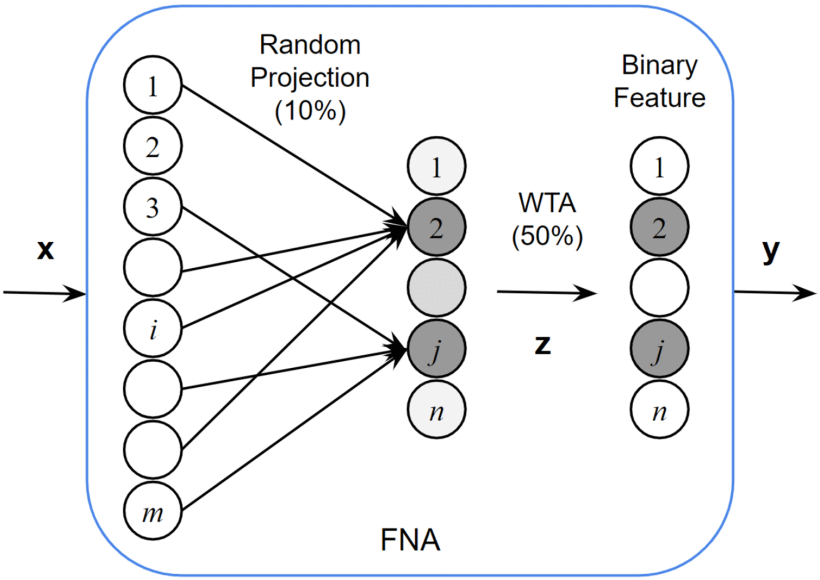
\includegraphics[width=0.7\linewidth]{images/fly.png}
\caption{The fly algorithm's network architecture. The random projection is shown only for the connection between the two hidden layer, but all the input layer is connected to the first hidden layer using the same mechanism}
\end{figure}

\subsubsection{FlyNet models}\label{header-n193}

The authors implement a range of VPR models, using FNA and a module with
temporal filtering capabilities. These networks models are the
following:

\begin{itemize}
\item
  \textbf{FlyNet:} it's composed by the FNA that terminates with a fully
  connected (FC) network. Its architecture is a three-layer MLP with
  64--64--1000 units respectively, where the first two layers make up
  the FNA and the last one composes the FC network.
\item
  \textbf{FlyNet+SeqSLAM:} it incorporates the SeqSLAM algorithm on top
  of our single-frame FlyNet network. This model can be compared along
  with the other following temporal models.
\item
  \textbf{FlyNet+RNN:} It is a purely neural model that incorporates an
  RNN on top of FlyNet and terminates with another FC layer. Its
  architecture is the same as FlyNet (the FC layers have 100 units),
  with 512 recurrent units. 
\item
  \textbf{FlyNet+CANN:} it incorporates a variation of the CANN
  architecture proposed in RatSLAM, which is a 1-dimensional model, on
  top of the FlyNet network. The CANN layer has 1002 units.
\end{itemize}

\begin{figure}[h!]
\centering
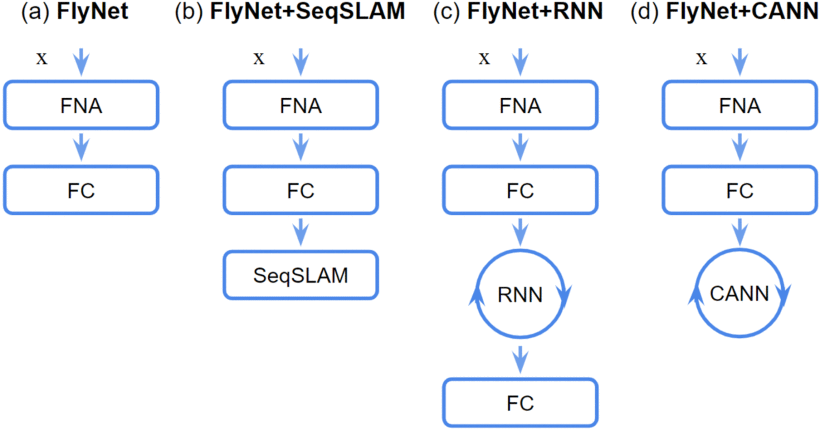
\includegraphics[width=0.8\linewidth]{images/flynetmodels.png}
\caption{FlyNet models}
\end{figure}

\subsection{Experiments}\label{header-n205}

\subsubsection{Dataset and data preprocessing}\label{header-n206}

To evaluate the capabilities of the proposed FlyNet-based models, the
authors conduct extensive experiments on two of the most widespread
benchmarks used in VPR, the \emph{Nordland} and \emph{Oxford RobotCar}
datasets. Nordland includes extreme seasonal changes across spring,
summer, fall, and winter, captured during a train journey, in northern
Norway. The summer traversal is used for training, and the remaining for
testing. The Oxford RobotCar dataset provides over 100 traverses with
different lighting (e.g. day, night) and weather (e.g. direct sun,
overcast) conditions through a car ride in Oxford city. The images are
pre-processed before being used by the models. FlyNet baselines convert
the images into single-channel (gray-scale) frames normalized between
{[}0, 1{]}, and then resize them to $32 \times 64$.

\subsubsection{Experiments evaluation}\label{header-n208}

The authors train and test the four FlyNet models in order to find the
best model and compare it with other existing state-of-the-art
techniques. In particular, these methods are \emph{SeqSLAM} (without FNA
attacked), \emph{LoST-X}, and \emph{Multi-Process Fusion}.

\paragraph{Metrics}\label{header-n210}

VPR models' performance is evaluated using precision-recall (PR) curves
and area under the curve (AUC) metrics. The tolerance used to consider a
query place as a correct match is being within 20 frames around the
ground truth location for the Nordland dataset, and up to 50 meters (10
frames) away from the ground truth for the Oxford RobotCar dataset.

\paragraph{Comparison of FlyNet to Other Neural
Networks}\label{header-n212}

FlyNet (alone) is compared with the other four single-frame models: a
simple FC network, an FC network with dropout, a CNN, and an
implementation of the NetVLAD method. The FC network has the same
architecture as FlyNet: it is a three-layer MLP with 64-64-1000 neurons
respectively. The FC network with dropout is the same as the previous
one, but with a dropout rate of 90\% and 50\% for the first and second
layers, respectively, in order to approximate the FlyNet sparsity and
for fair comparison purposes. The CNN model has 2 convolutional layers
while the NetVLAD output representation dimensionality is reduced from
4096 to 64 to be comparable in size with the FlyNet.
\newpage
\subsection{Experiments results}\label{header-n214}

\subsubsection{FlyNet vs. Other Single-Frame
Networks}\label{header-n215}

FlyNet is directly competitive with both FC networks, despite FlyNet
having over 3 times fewer parameters (64 k vs. 199 k). CNN and NetVLAD
models, with 6 and 234 times more parameters than FlyNet respectively,
the larger the model the better the results we obtained. Under
\emph{small environmental changes} (e.g. summer to fall) both networks
achieved over 70\% AUC. However, under \emph{extreme visual changes}
(e.g. summer to winter) all these models show relatively similar
results, below 12\% AUC, except for NetVLAD with 20\% AUC.

\begin{figure}[h!]
\centering
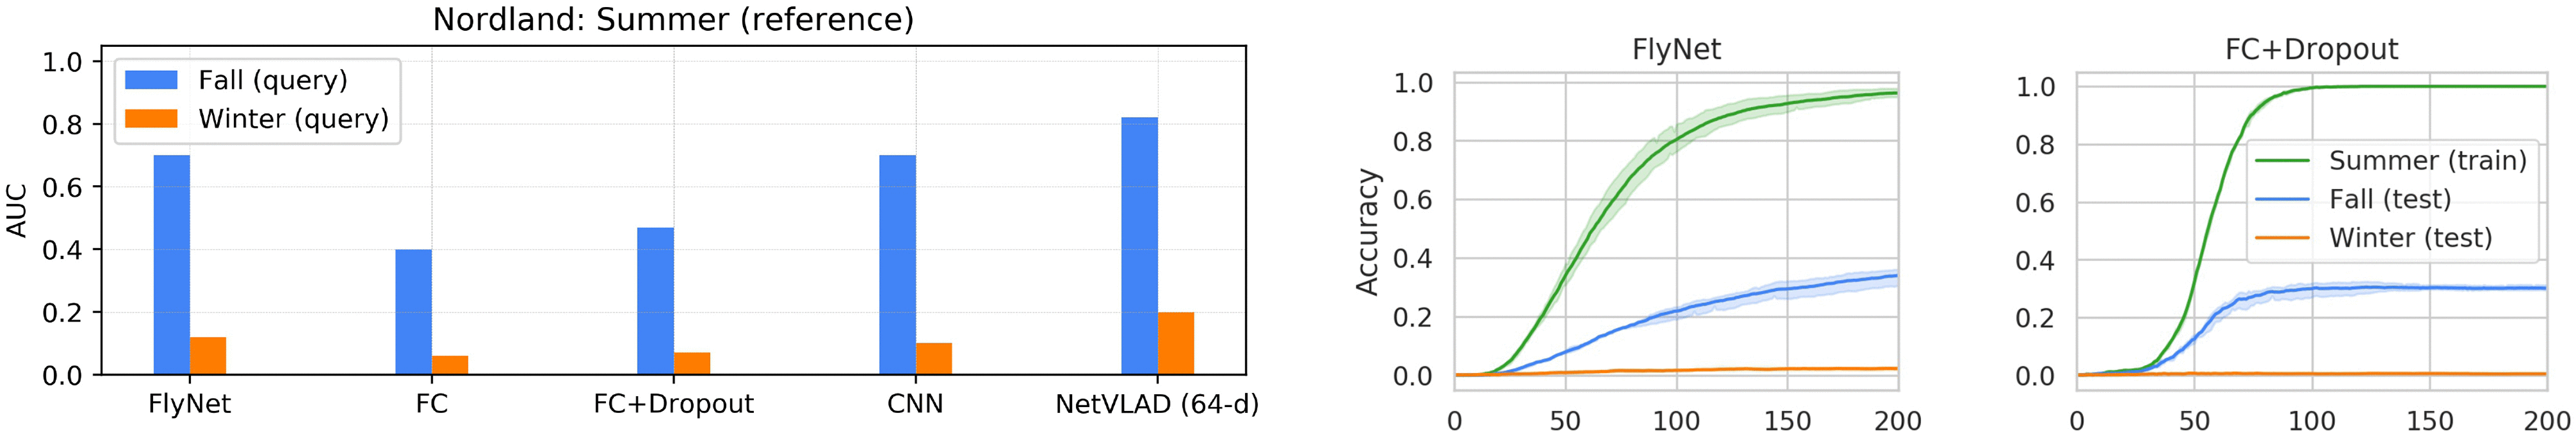
\includegraphics[width=\linewidth]{images/flynetothermodels.png}
\caption{Comparison of FlyNet (alone) to other single-frame neural networks. AUC results across different models on the Nordland dataset (left). Average accuracy over 10 training experiments vs. number of epochs for FlyNet (middle) and a fully connected (FC) network with dropout (right).}
\end{figure}

\subsubsection{FlyNet models evaluation}\label{header-n218}

Although there are significant performance differences at a single-frame
matching level, the figure below shows that when using sequence-based
filtering techniques these differences reduce significantly. For
FlyNet+SeqSLAM, the performance of FlyNet (alone) was significantly
improved. Similarly, the RNN layer on top of FlyNet improved even
further these results. However, when integrating the output of FlyNet
with a 1-d CANN we were able to outperform these models, even under
extreme environmental changes: this is the best model.

\begin{figure}[h!]
\centering
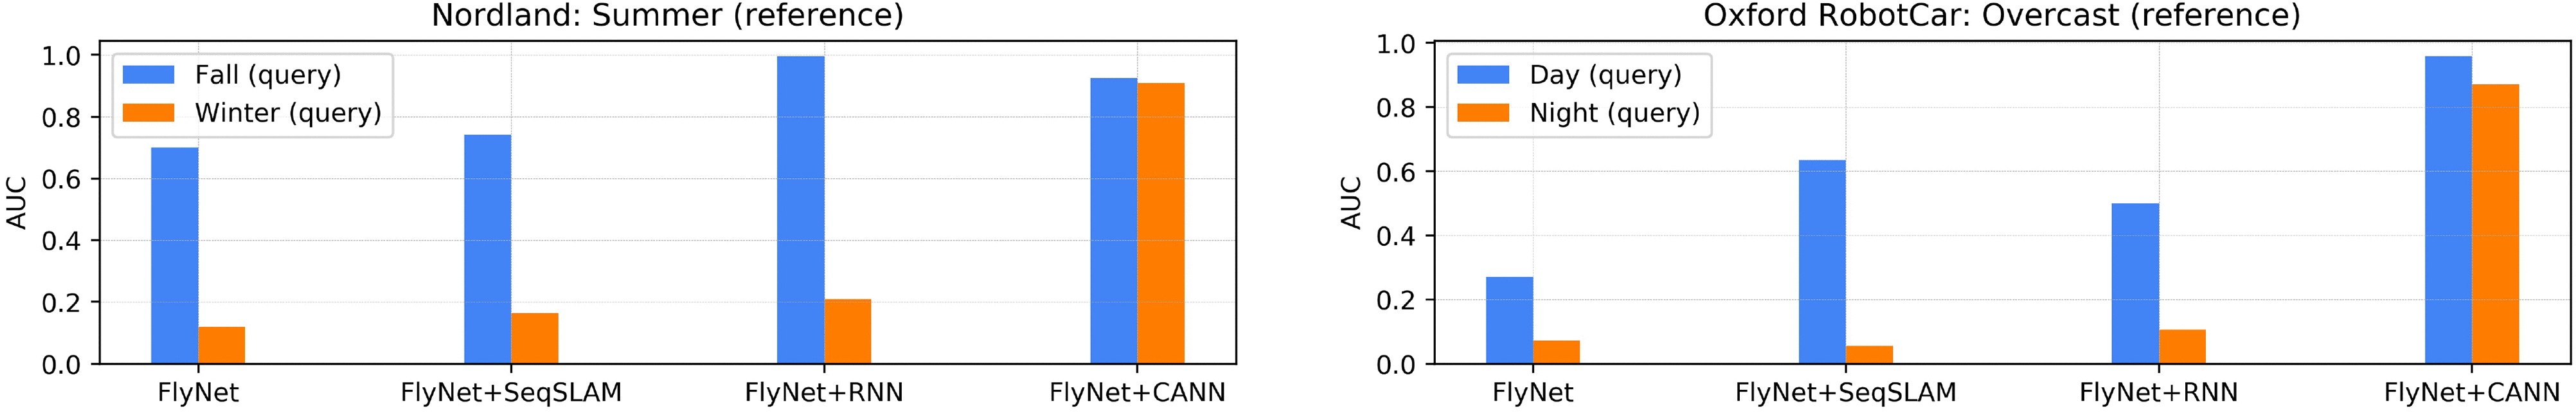
\includegraphics[width=1\linewidth]{images/flynetcomparemodels.png}
\caption{AUC results of the four FlyNet models}
\end{figure}

\newpage

\subsubsection{Best model vs. state-of-the-art
methods}\label{header-n221}

MPF is performing better while being able to recall almost all places at
100\% precision on both fall and winter testing traverses. FlyNet+CANN
achieves state-of-the-art results, comparable with SeqSLAM and MPF in
all these tested traverses.

\begin{figure}[h!]
\centering
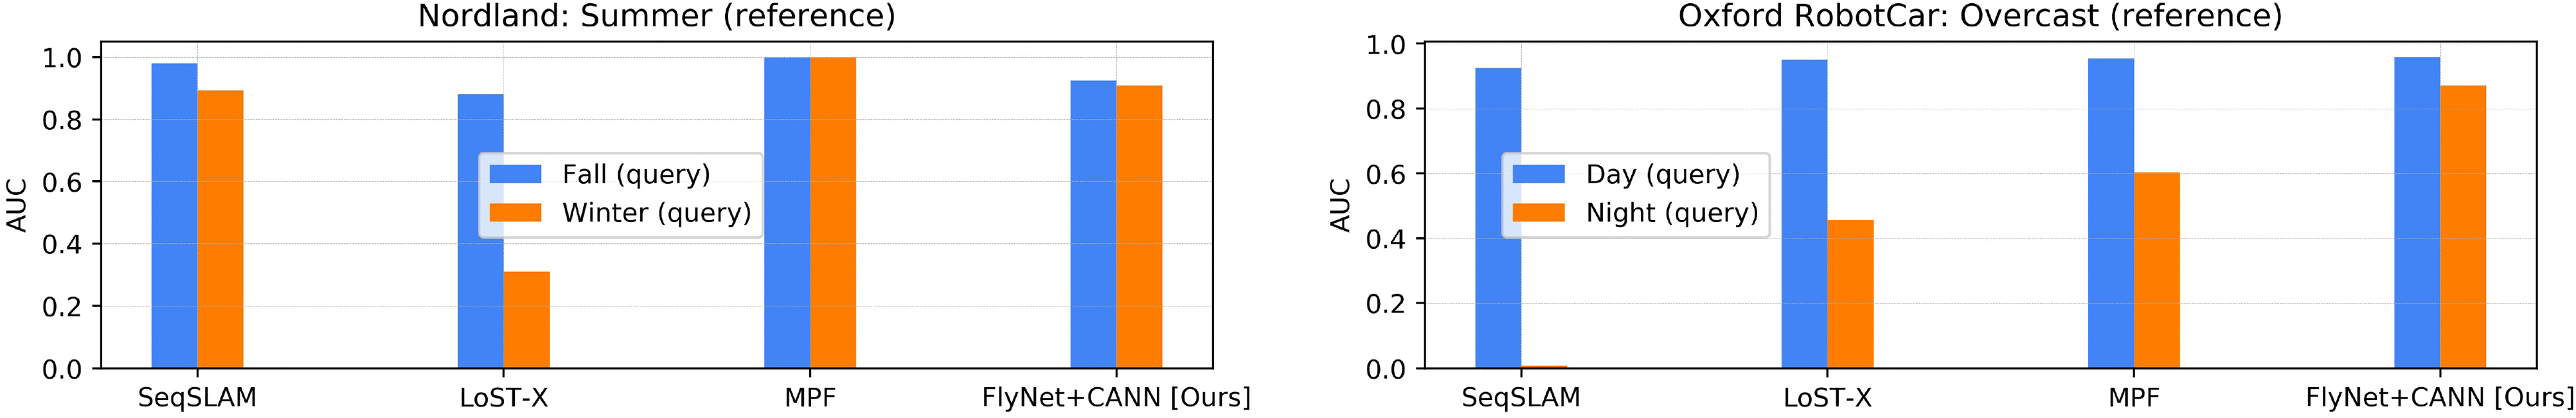
\includegraphics[width=1\linewidth]{images/bestmodelvsothers.png}
\caption{AUC results of the state-of-the-art methods measured on the two dataset}
\end{figure}

Similarly, PR performance on the Oxford RobotCar dataset is shown in the
following figure. FlyNet+CANN not only achieves state-of-the-art results
comparable with the other methods, but it maintains PR performance even
under extreme environmental changes (e.g. overcast to night), as shown
the bottom-right side of the figure.

\begin{figure}[h!]
\centering
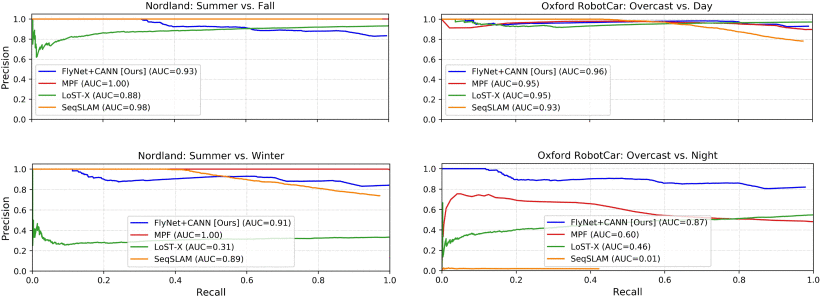
\includegraphics[width=1\linewidth]{images/bestmodelvsothersPR.png}
\caption{PR results of the state-of-the-art methods measured on the two dataset}
\end{figure}

\subsubsection{Computational performance}\label{header-n226}

The processing time required to perform appearance-invariant VPR by our
hybrid model is compared to those from state-of-the-art methods in terms
of running time for (1) feature extraction, (2) visual place matching
between query and reference traverses, and (3) average place recognition
time for a single query image from a 1000-image reference database. This
Avg. Time (3) is calculated as (Feature Ext. (1) + Place Match.
(2))/1000. Processing time results on the Nordland dataset are reported
in the following table. The FlyNet+CANN can be up to 6.5, 310, and 1.5
times faster than MPF, LoST-X, and SeqSLAM, respectively.

\begin{longtable}[]{@{}llll@{}}
\toprule
\textbf{Method} & \textbf{Feature extraction} & \textbf{Place matching}
& \textbf{Avg. time (fps)}\tabularnewline
\midrule
\endhead
\textbf{FlyNet+CANN} & \textbf{35 sec} & \textbf{25 sec} & \textbf{0.06
sec (16.66)}\tabularnewline
MPF & 1.9 min & 4.6 min & 0.39 sec (2.56)\tabularnewline
LoST-X & 110 min & 200 min & 18.6 sec (0.05)\tabularnewline
SeqSLAM & 50 sec & 40 sec & 0.09 sec (11.11)\tabularnewline
\bottomrule
\caption{Processing time comparison on the Nordland dataset}
\end{longtable}

The following figure shows the comparison between the networks'
complexity and the results obtained, viewing the AUC metric for the most
challenging appearance change (day to night). The best model proposed in
this works obtains the best results with the minimum number of
parameters.

\begin{figure}[h!]
\centering
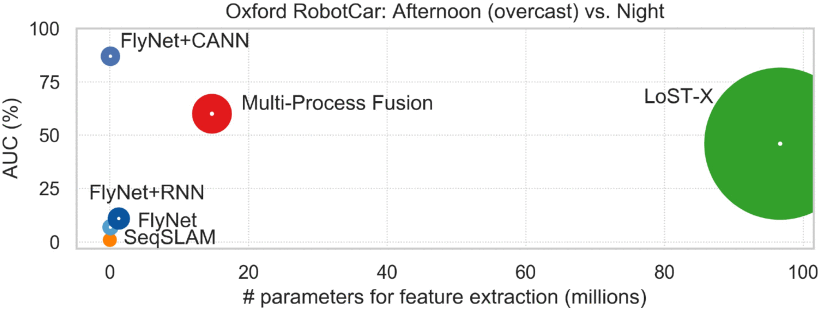
\includegraphics[width=1\linewidth]{images/flynetothermodeldimensions.png}
\caption{Oxford RobotCar AUC performance vs. Network Size. Comparison for the most challenging appearance change (day to night)}
\end{figure}

\subsection{Conclusions}\label{header-n256}

FlyNet+CANN model achieves competitive visual localization results
compared to existing deep learning and algorithmic-based VPR techniques,
but with significantly fewer parameters, a smaller footprint, and
reduced processing time. The authors want to demonstrate that, taking
inspiration from the biological brain, it is possible to build
sample-efficient, high-performing VPR models. FlyNet has the same number
of layers and sparse structure found in the fly olfactory neural
circuit. Despite the fly, brains extend by forty times the
dimensionality of the inputs, the authors have experimentally shown that
also reducing this dimension the FlyNet training accuracy remained
around 96\%. At the same time, FlyNet+CANN enabled the use of a
relatively low-performance but fast network to get better VPR results,
which is also able to generalize across challenging environmental
changes.
\newpage

\section{A Multimodal Target-Source Classifier With Attention Branches
to Understand Ambiguous Instructions for Fetching Daily
Objects}\label{header-n258}

\emph{IEEE ROBOTICS AND AUTOMATION LETTERS, VOL. 5, NO. 2, APRIL 2020}
{[}29{]}

\subsection{Introduction}\label{header-n260}

In the last few years, the domestic service robots (DSRs) have become
more popular: they have a lot of different and useful functions and they
can help people with disabilities. Despite this, one of the main
limitations of DSRs is their inability to naturally interact through
natural language. This ability may be appreciated by non-expert users. A
particular task like various expressions relating to an object for
fetching tasks. This work focuses on \emph{multimodal language
understanding for fetching instructions} (MLU-FI). This task consists of
predicting a target instructed in natural language, such as ``\emph{Bring
me the yellow box from the wooden cabinet.}". The purpose is to
understand how to extract instructions for robots from natural-language
expressions. Natural language induces ambiguity because of the
many-to-many mapping between the linguistic and physical world which
makes it difficult to accurately infer the user's intention. In this
work, the authors propose the multimodal target-source classifier model
with the attention branch (MTCM-AB) which is an extension of the MTCM
(proposed in {[}5{]}), with the addition of the attention branch network
(ABN) explained in {[}6{]}. The MTCM module predicts the region-wise
likelihood of target and source candidates in the scene. Unlike other
methods, MTCM can handle region-wise classification based on linguistic
and visual features. The ABN is an image classifier, inspired by class
activation mapping (CAM) structures, that generates attention maps. This
line of research focuses on the production of image masks that, overlaid
onto an image, highlight the most salient portions with respect to some
given query or task. An attention map is an image with highlighted the
salient regions of a given label. Multiple visual attention networks
were also proposed in recent years for solving visual question
answering. However, most of these approaches use only a single modality
for attention: visual attention. By contrast, recent studies in
multimodal language understanding have shown that both linguistic and
visual attention is beneficial for the given task.

\subsection{Problem definition}\label{header-n262}

The aim is to predict a target referred by an initial instruction among
a set of candidate targets in a visual scene. Instructions are not
constrained which is more natural but increases the complexity of the
comprehension task because users may use referring expressions to
characterize a target. Examples of possible instruction can be:
``\emph{Take the Kleenex box and put it in the bottom right box}" or
``\emph{Go to the kitchen and take the tea bottle on the upper shelf}".
To address the MLU-FI are considered:

\begin{itemize}
\item
  \textbf{Input:} a fetching instruction as a sentence in addition to an
  image of the scene. 
\item
  \textbf{Output:} the most likely target-source pair. The terms target
  and source are defined as follows.

  \begin{itemize}
  \item
    \textbf{Target:} a daily object (e.g. bottle or snacks) that a user
    intends the robot to fetch.
  \item
    \textbf{Source:} the origin of the target (e.g. desk or cabinet).
  \end{itemize}
\end{itemize}

The evaluation metric is the prediction accuracy over the top-1 target
prediction. Ultimately this study does not focus on object detection.
The authors suppose that the bounding boxes of the target and source are
given in advance. The MTCM-AB is not specifically designed for a given
scene or context. It is validated on two types of datasets, in real and
simulated environments described below.

\begin{itemize}
\item
  \textbf{Home Environment:} In this configuration, the experiments use
  a simulation-based dataset from the Partner Robot Challenge Virtual
  Space (WRS-PV). WRS-PV depicts home environments as represented in the
  figure below. The three-dimensional environments (Unity-based) are
  augmented to make them more realistic. In this environment, a targeted
  DSR, that is HSR (Human Support Robot), can freely navigate and
  manipulate objects. In this context, the MTCM-AB predicts the most
  likely target among several candidates.
\item
  \textbf{Pick-and-Place Scene:} the PFN-PIC {[}7{]} dataset is designed
  for pick-and-place tasks from an armed robot with a top-view camera.
  The scene consists of four boxes, in which several candidate targets
  (up to 40) are randomly placed.
\end{itemize}

\begin{figure}[h!]
\centering
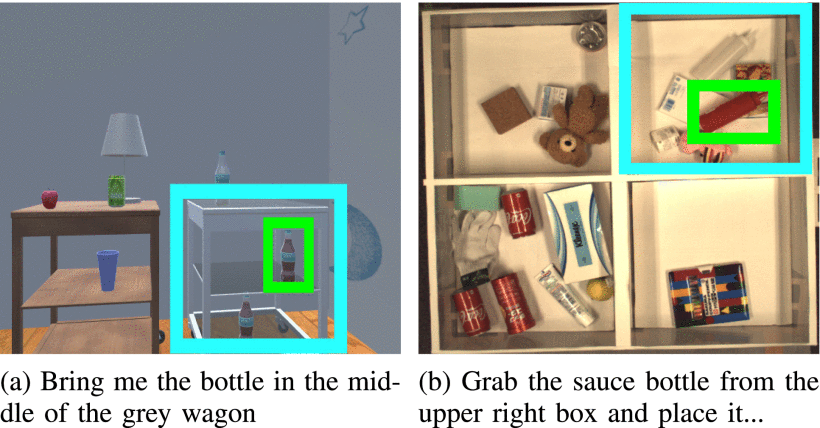
\includegraphics[width=0.8\linewidth]{images/WRS-PVexample.png}
\caption{Samples of the WRS-PV (left) and PFN-PIC datasets (right) where the source and target are given.}
\end{figure}

\subsection{Proposed method}\label{header-n281}

The proposed method consists of target prediction with respect to
instruction in natural language. The authors extend the MTCM {[}5{]}
with an attention branch network (ABN, {[}6{]}) that are used to improve
the prediction from the linguistic and visual inputs. In ABN, the class
attention map (CAM) network is extended to produce an attention mask for
improving image classification. The ABN is decomposed into parallel
branches to avoid deteriorating the classifier accuracy (both of them
are classifiers):

\begin{itemize}
\item
  an attention branch that produces attention maps and
\item
  a prediction branch that predicts the likelihood of some label.
\end{itemize}

The MTCM-AB module produced in this work, similarly to the MTCM,
predicts the target and source from the full sentence. This module is
composed of a set of sub-modules: the Target Attention Branch (TAB), the
neighboring Context Attention Branch (nCAB), and the Linguistic
Attention Branch (LAB). The MTCM-AD architecture is explained in detail
in the following line and the figure below is a visual representation of
it. The MTCM module works as follow:

\begin{itemize}
\item
  \textbf{Input:} for each target candidate $i \in \{1, . . ., N\}$
  and source $i^{'} \in \{1, . . ., M\}$, the input is

  $ {\mathbf x}(i)=\lbrace {\mathbf x}_{l}(i), {\mathbf x}_{t} (i), {\mathbf x}_{c} (i), {\mathbf x}_{r} (i) \rbrace, $

  where ${\mathbf x}_l(i)$, ${\mathbf x}_t(i)$, ${\mathbf x}_c(i)$ and
  ${\mathbf x}_r(i)$ denote linguistic, target, context and relation
  features. The authors purposefully omit index in the following, that
  is, ${\mathbf x}(i)$ is then written as ${\mathbf x}$. More in detail, the
  input variables define:

  \begin{itemize}
  \item
    ${\mathbf x}_t(i)$: it is defined as the cropped image of the target
  \item
    ${\mathbf x}_c(i)$: it is a cropped image that characterizes a target
    and its neighborhood (context)
  \item
    ${\mathbf x}_c(l)$: it consists of sub-word vector embedding
  \item
    ${\mathbf x}_r(i)$: it is a vector characterizing the position of the
    target candidate in the environment.
  \end{itemize}
\item
  \textbf{Linguistic Attention Branch (LAB):} its purpose is to
  emphasize the most salient part of the linguistic features for
  instruction comprehension. The LAB module is composed by a
  implementation of the BERT method for the sub-word embedding (extract
  the words internal structure). Subsequently, the multi-layer Bi-LSTM
  network is used to obtain a latent space representation of the
  extracted linguistic features. The last hidden states of each layer
  are concatenated to form \emph{linguistic feature maps}
  f\textsubscript{l}, from which a linguistic attention mask is
  extracted. Feature maps f\textsubscript{l} are processed through
  one-dimensional convolutional layers followed by a single fully
  connected layer (FC) The \emph{linguistic attention map}
  a\textsubscript{l} is obtained from the second convolutional layer
  that is convoluted with an additional layer and normalized by a
  sigmoid activation function. The output visual feature maps are then
  obtained using a masking process given by

  $ {\mathbf o}_{l}= {\mathbf a}_l \odot {\mathbf f}_{l} $

  where $\odot$ denotes the Hadamard product (takes two matrices of
  the same dimensions and produces another matrix of the same dimension
  as the operands where each element $i, j$ is the product of elements
  $i, j$ of the original two matrices).
\item
  \textbf{Target Attention Branch (TAB):} it produces an attention map
  for the candidate target images. The input ${\mathbf{x}_t}$ is
  transformed into a space feature ${\mathbf{f}_t}$ through a CNN, which
  is processed into FC layers. Even in this case, a visual attention map
  is extracted from the second FC layer that is processed in a parallel
  branch composed of a FC layer and a sigmoid activation function.
  Output latent space feature o\textsubscript{t} is then obtained by

  $ {\mathbf o}_{t}= {\mathbf a}_t \odot {\mathbf f}_{t}.$
\item
  \textbf{Neighboring Context Attention Branch: (nCAB):} it is one of
  the main novelties of the MTCM-AB. nCAB module adds an attention
  branch mechanism to focus on the relevant part of the image in the
  surroundings of a given target, in order to define context features.
  An extended cropped image (${\mathbf x}_c$) is extracted from around the
  target. This input is encoded into feature maps ${\mathbf{f}_c}$ from a
  CNN feature extractor. The convolutional layers are followed by a
  global average pooling (GAP). In parallel, context attention map
  a\textsubscript{c} is created from an additional convolution and
  sigmoid normalization of the third convolutional layer. The output
  context feature maps are given by

  $ {\mathbf o}_{c}= {\mathbf a}_{c} \odot {\mathbf f}_{c}.$
\item
  \textbf{Perception Branch:} it is composed by a visual multi-layer
  perceptron (MLP), which encodes the concatenation of ${\mathbf{o}_t}$,
  ${\mathbf{o}_v}$ and ${\mathbf{x}_r}$. In parallel, a linguistic MLP
  encodes linguistic features ${\mathbf{o}_l}$. The source is predicted as
  ${\mathbf{J}_{src}}$ from a third MLP that combines the two previous MLP
  outputs.
\item
  \textbf{Loss Functions:} the MTCM-AB is trained by minimizing several
  embedding loss functions related to the different branches. In
  particular, it minimizes the global loss function
  $J_{total} = \lambda_cJ_c + \lambda_tJ_t + \lambda_lJ_l + \lambda_pJ_p + \lambda_{src}J_{src}$,
  where J\textsubscript{i} is the loss function for the branch i and
  $\lambda_i$ are loss weights that are defined in the experimental
  section.
\end{itemize}

\begin{figure}[h!]
\centering
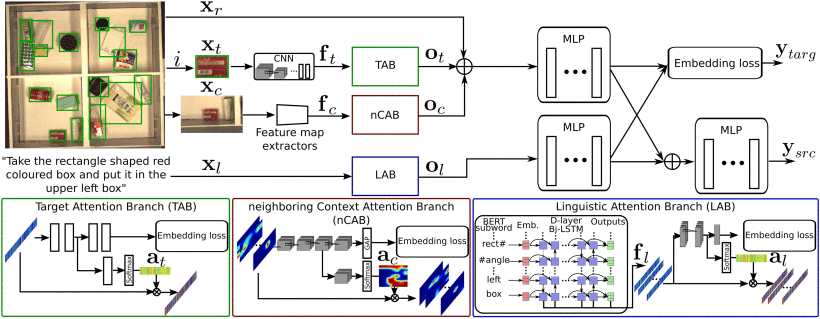
\includegraphics[width=0.8\linewidth]{images/MTMC-AB.png}
\caption{MTCM-AB architecture}
\end{figure}

\subsection{Experiments}\label{header-n318}

The proposed method is evaluated over the PFN-PIC and WRS-PV datasets.
The first contains 89,891 sentences in the training set and 898
sentences in the validation set to instruct 25,861 targets in the
training set and 532 targets in the validation one. The latter, instead,
has 308 images from which 2015 instructions in the training set and 74
instructions in the validation set. The experimental setup is summarized
in the following figure. This configuration is used to train the model
with the PFN-PIC dataset, while for the WRSPV dataset the learning rate
was decreased to $5 \times 10^{-5}$ and a batch size of 64.

\begin{figure}[h!]
\centering
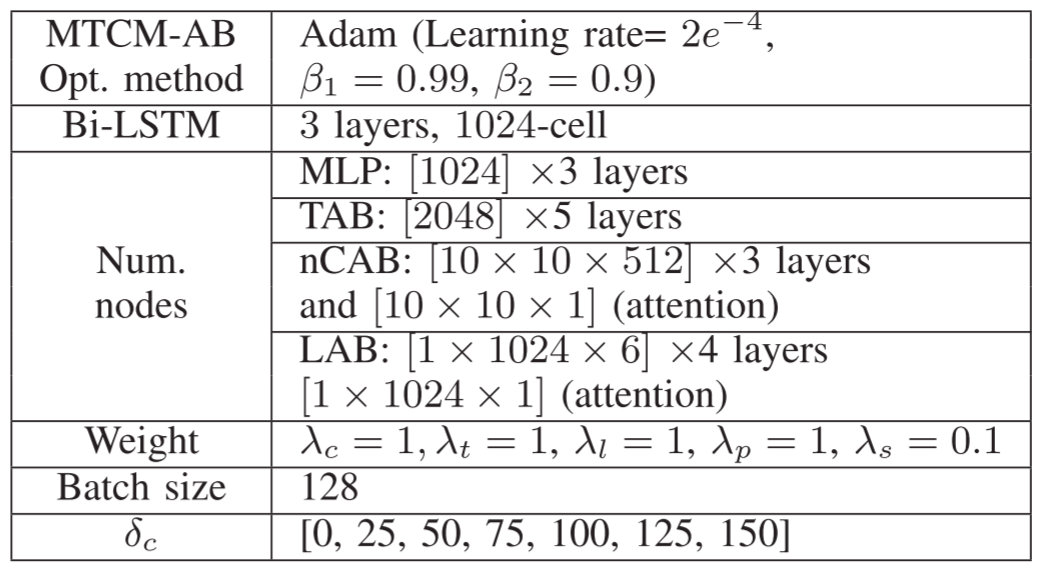
\includegraphics[width=0.85\linewidth]{images/MTCMsettings.png}
\caption{MTCM-AB settings parameters}
\end{figure}

The input images were downscaled to $299 \times 299$ before being processed.
The parameter $\delta_c$ represents the variation in size of the
context input ${\mathbf x}_c$. It corresponds to the size of the cropped
image target to which is added $\delta_c$ in width and height. The
MTCM-AB had 27.5 M parameters.

\newpage
\subsection{Results}\label{header-n322}

\subsubsection{Quantitative results}\label{header-n323}

The \emph{quantitative results} correspond to the accuracy obtained for
the most likely target predicted, given an instruction. This metrics is
also called \emph{top-1 accuracy}. The authors report the performance
variation with varying sizes of ${\mathbf x}_c$ by setting $\delta_c$
with a 0 to 150-pixel wise extension, to find the best value of.
$\delta_c$These results are reported in the following figure.

\begin{figure}[h!]
\centering
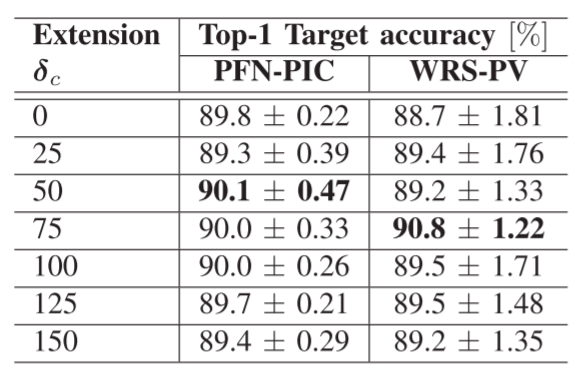
\includegraphics[width=0.65\linewidth]{images/MTCMresultssize.png}
\caption{MTCM-AB accuracy with respect to $\delta_c$}
\end{figure}

From $\delta_c$ analysis, the authors found its best value for the two
datasets, which is, respectively, 50 and 75 pixels for the PFN-PIC and
WRS-PV datasets. In addition, this analysis shows that the PFN-PIC
dataset is highly cluttered with relatively small objects, because
setting $\delta_c = [125, 150]$ causes lower accuracy than the
configuration with $\delta_c = 0$. The MTCM-AB method proposed in this
work is compared with respect to other state-of-the-art models and human
performance, which is considered as an upper bound. These confront
models are the MTCM {[}1{]} and its baseline method explained in {[}7{]}
by Hatori et al. The results, in terms of top-1 accuracy, are reported
in the following figure.

\begin{figure}[h!]
\centering
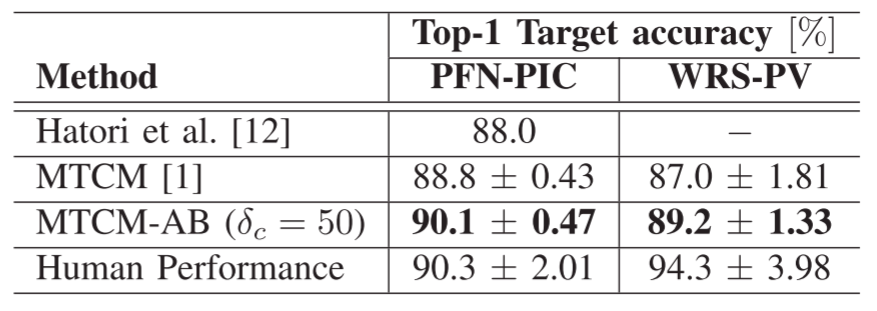
\includegraphics[width=0.75\linewidth]{images/MTCMqualres.png}
\caption{Top-1 Accuracy on PFN-PIC and WRS-PV datasets}
\end{figure}

On PFN-PIC, the MTCM-AB outperformed the MTCM and baseline method by
1.3\% and 2.1\% respectively. The results of WRS-PV corroborated the
trend observed on the PFN-PIC dataset. To characterize the contribution
of each attention branch, the authors also report the results of an
ablation study for the PFN-PIC dataset. These results, showed in the
following figure, show that both linguistic and visual attention
branches improved the prediction accuracy compared to the MTCM.

\begin{figure}[h!]
\centering
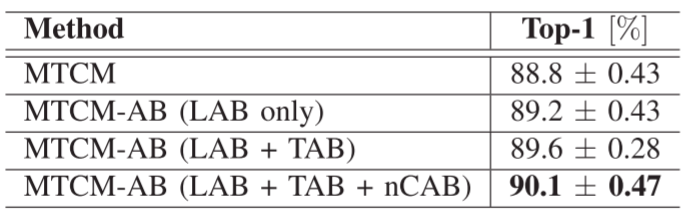
\includegraphics[width=0.75\linewidth]{images/MTCMablanation.png}
\caption{Ablanation study of the MTCM-AB for PFN-PIC dataset}
\end{figure}

\subsubsection{Qualitative Results}\label{header-n330}

In the following figure, the \emph{qualitative results} are reported for
the PFN-PIC dataset. In the first row, the prediction is given in blue
while the ground truth is in green. The attended region of each context
feature ${\mathbf x}_c$ is given in the second row. The two first columns
refer to correct predictions. The third column refers to an erroneous
prediction (wrongly attended target), while the last column refers to an
erroneous prediction due to incorrect ground truth (``brown pack is
instructed but ``can is given the label). The sentences are:

\begin{itemize}
\item
  ``\emph{Take the blue sandal move it to lower left box}
\item
  ``\emph{Take the green item next to the pair of white gloves and move
  it to top left box}
\item
  ``\emph{Move the grey colored bottle at top left to box below}.
\item
  ``\emph{Pick the brown pack and put it in lower left box}
\end{itemize}
\newpage
\begin{figure}[h!]
\centering
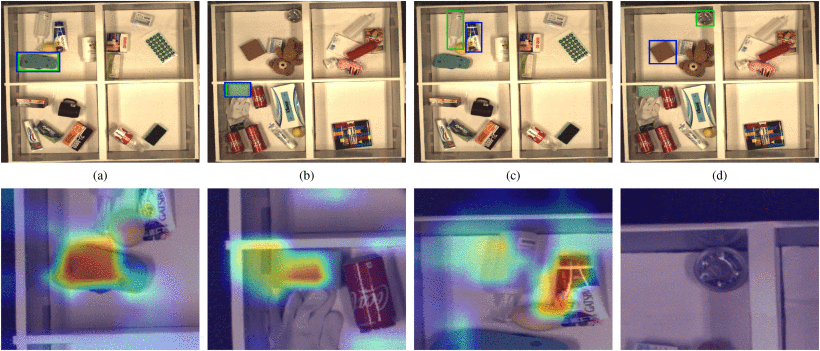
\includegraphics[width=0.8\linewidth]{images/MTMCqualres1.png}
\caption{Qualitative results for PFN-PIC dataset}
\end{figure}

Qualitative results on the WRS-PV dataset are analyzed in the same way.
The three first samples illustrate correct predictions with consistent
attended regions. The last sample, with the instruction ``Take an apple
on the same shelf that a coffee cup is placed is erroneous and our
model predicts the cup instead of the apple.

\begin{figure}[h!]
\centering
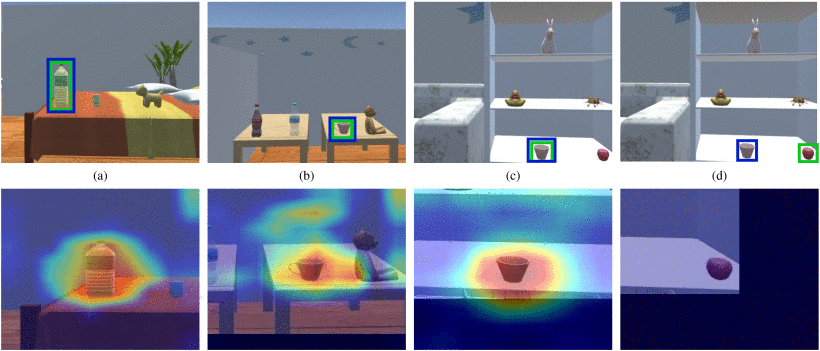
\includegraphics[width=0.8\linewidth]{images/MTMCqualres2.png}
\caption{Qualitative results for WRS-PV dataset}
\end{figure}

\subsubsection{Error Analysis}\label{header-n344}

Analysing the MTCM-AB results, different failure cases can be observed:

\begin{itemize}
\item
  \textbf{ES (erroneous sentence):} the ground truth does not correspond
  to the target specified in the instruction
\item
  \textbf{NE (negation):} the ground truth is specified from a negation
  sentence which is thought to be difficult to solve in NLP community
\item
  \textbf{REL (relation to landmark):} the ground truth is defined with
  respect to landmark objects and the predicted target position is
  incorrect with respect to this landmark
\item
  \textbf{RES (relation to source):} the ground truth target is defined
  with respect to a source and the predicted target position is
  incorrect with respect to this source
\item
  \textbf{SE (source error):} the instruction specifies a given source
  and the predicted target position is in a different source
\end{itemize}
\newpage

\section{CNN Based Road User Detection Using the 3D Radar
Cube}\label{header-n359}

\emph{IEEE ROBOTICS AND AUTOMATION LETTERS, VOL. 5, NO. 2, APRIL 2020}
{[}8{]}

\subsection{Introduction}\label{header-n361}

Radars are attractive sensors for intelligent vehicles as they are
relatively robust to weather and lighting conditions (e.g. rain, snow,
darkness) compared to camera and LIDAR sensors. They also have excellent
range sensitivity and can measure radial object velocities directly
using the Doppler effect. A radar outputs a point-cloud of reflections
called \emph{radar targets} in every frame and each radar target has the
following features: range $r$ and azimuth $\alpha$, radar cross
section RCS (i.e. reflectivity), and the object's radial speed $v_r$
relative to the ego-vehicle. The authors call these feature
\emph{target-level}. Many radar-based road user detection methods first
cluster radar targets by their \emph{target-level} features. Object
detection and classification methods depend on the success of this
initial classification step. Other methods explore using the
\emph{low-level radar cube} given by early processing of the radar
signal. The radar cube is a 3D data matrix with axes corresponding to
range, azimuth, and velocity (also called Doppler). In contrast to the
target-level data, the radar cube provides the complete speed
distribution (i.e. Doppler vector) at multiple 2D range-azimuth
locations. Such distributions can capture modulations of an object's
main velocity caused by its moving parts, e.g. swinging limbs or
rotating wheels. In this work, the authors show that these data can be
used as valuable features for object classification. The features
derived from a 3D cube are called \emph{low-level}. This work focus only
on addressing moving road users. In \emph{Prophet}, proposed in
{[}10{]}, radar targets are first clustered into objects by DBSCAN.
Then, several cluster-wise features are extracted, e.g. the
variance/mean of $v_r$ and $r$. The performance of various
classifiers (Random Forest, Support Vector Machine (SVM), 1-layer Neural
Network, etc.) were compared in a single-class (pedestrian) detection
task. The Schumann method {[}11{]} also uses clusters calculated by
DBSCAN as the base of a multi-class (car, pedestrian, group of
pedestrians, cyclist, truck) detection, but extract different features,
e.g. deviation and spread of α (azimuth). In this letter, the authors
propose a radar-based, multi-class moving road user detection method,
which exploits both expert knowledge at the \emph{target-level}
(accurate 2D location, addressed phase ambiguity), and \emph{low-level}
information from the full 3D radar cube rather than a 2D projection. The
method's core is a Convolutional Neural Network (CNN) called Radar
Target Classification Network (\emph{RTCnet}). The inclusion of
low-level data enables the classification of individual radar targets
before any object clustering; the latter step can benefit from the
obtained class scores.

\subsection{Proposed method}\label{header-n363}

\emph{RTCnet} classifies each target individually based on the fused
low-level and target-level data. The network consists of three parts.
The first encodes the data in spatial domains (range, azimuth) and
grasps the surroundings' Doppler distribution. The second is applied to
this output to extract class information from the distribution of speed.
Finally, the third part provides classifications scores by two fully
connected layers (FC). The output is either multi-class (one score for
each class) or binary. In the latter case, an ensemble voting step
combines the result of several binary classifiers. A class-specific
clustering step (i.e. the radar targets' predicted class information is
used) generates an object list output. The following figure shows an
overview of our method.

\begin{figure}[h!]
\centering
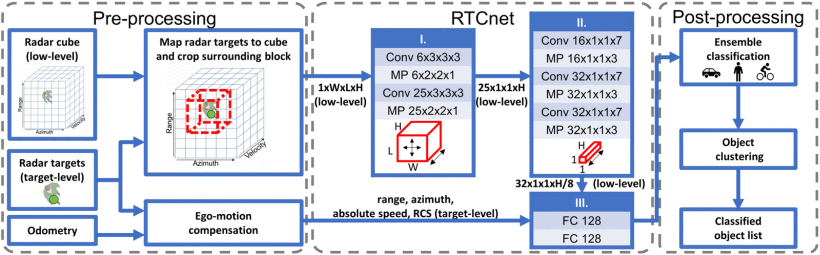
\includegraphics[width=0.95\linewidth]{images/pipelineoverview.png}
\caption{The proposed pipeline's architecture}
\end{figure}

\subsubsection{Pre-Processing}\label{header-n366}

Every single frame of radar targets and a single frame of the radar cube
(low-level data) is fetched and pre-processed. First, radar targets with
low compensated (absolute) velocity are considered as static and are
filtered out. Then, corresponding target-level and low-level radar data
are connected. Next, we look up each remaining dynamic radar target,
such as a grid cell in the radar cube based on their reported range,
azimuth, and (relative) velocity ($r$, $\alpha$, $v_r$).
Afterward, a 3D block of the radar cube is cropped around each radar
target's grid cell with radius in range/azimuth/Doppler dimensions
($L$, $W$, $H$).

\subsubsection{Network}\label{header-n368}

The \emph{RTCnet} structure can be seen in detail in the figure above.
The network is composed of three modules:

\begin{itemize}
\item
  \textbf{Down-Sample Range and Azimuth Dimensions:} it aims to encode
  the radar target's spatial neighborhood's Doppler distribution into a
  tensor without extension in range or azimuth. In other words, it
  transforms the $1 \times W \times L \times H$ sized data to a $C \times 1 \times 1
  \times H$ sized tensor (sizes are given as $Channel \times Azimuth \times Range \times
  Doppler$), where $C$ was chosen as 25. To do this, it contains two 3D
  convolutional layers (Conv) followed by two maxpool layers (MP).
\item
  \textbf{Process Doppler Dimension:} the aim of this module is to
  extract class information from the speed distribution around the
  target. It operates on the output of the first which is $25 \times 1 \times 1 \times
  H$. To do this, two 1D convolutions along the Doppler dimension are
  applied, each of them is followed by a maxpool layer. The output of
  this module is a $32 \times 1 \times 1 \times H/8$ block.
\item
  \textbf{Score Calculation:} The output of the second module is
  flattened and concatenated to the \emph{target-level} features ($r$,
  $\alpha$, $v_r$, $RCS$) and used by this module. It uses two
  fully connected layers with 128 nodes each to provide scores. The
  output layer has either four nodes (one for each class) for
  multi-class classification or two for binary tasks.
\end{itemize}

\subsubsection{Ensemble Classifying}\label{header-n377}

It is possible to train the third module to perform multi-class
classification directly. It implements also an ensemble voting system of
binary classifiers, in the case of the network has two output nodes.
This module is trained as One-vs-All (OvA) and One-vs-One (OvO) binary
classifiers for each class (e.g. car-vs-all) and pair of classes (e.g.
car-vs-cyclist), 10 in total.

\subsubsection{Object Clustering}\label{header-n379}

To obtain proposals for object detection, the authors cluster the
classified radar targets with DBSCAN incorporating the predicted class
information. The radar targets with bike/pedestrian/car predicted labels
are clustered in separate steps. As a metric, we used a spatial
threshold $\gamma_{xy}$ on the Euclidean distance in the $x, y$
space, and a separate speed threshold $\gamma_v$ in velocity
dimension. The advantage of clustering each class separately is that no
universal parameter set is needed for DBSCAN. The authors use different
parameters for different classes, e.g. larger radius for cars and small
ones for pedestrians. Furthermore, swapping the clustering and
classification step makes it possible to consider objects with a single
reflection. The following figure reports three challenging cases for the
cluster classification:

\begin{itemize}
\item
  \textbf{A:} objects may be clustered together (red circle)
\item
  \textbf{B:} large objects may be split up into several clusters
\item
  \textbf{C:} object with only one reflection
\end{itemize}

\begin{figure}[h!]
\centering
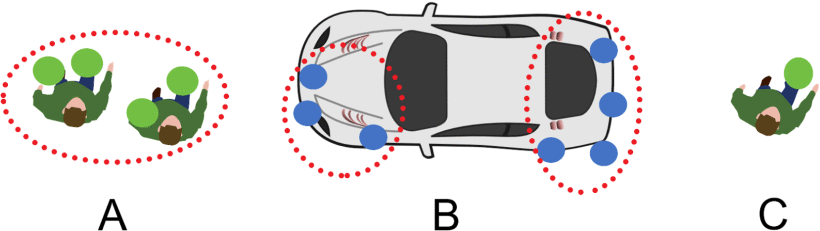
\includegraphics[width=0.95\linewidth]{images/clusteringdiff.png}
\caption{Challenging cases for cluster-wise classification methods}
\end{figure}

To address this, the method performs a filtering on the produced object
proposals, calculating their spatial, velocity, and class score
distribution distances. If two clusters have different classes and are
close enough in all dimensions, they are merged the smaller class to the
larger (i.e. pedestrians to cyclists and cars, cyclists to cars).

\subsubsection{Dataset}\label{header-n390}

The dataset is obtained in the real-world with a demonstration vehicle
during a time of an hour. There are recorded both the target-level and
low-level output of our radar, the output of a stereo camera ($1936 \times
1216$ px), and the vehicle's odometry (filtered location and ego-speed).
Annotation was fetched automatically from the camera sensor using the
Single Shot Multibox Detector (SSD) {[}9{]}. Then, the mislabeled ground
truth are corrected manually. To further extend the training dataset,
the authors augmented the data by mirroring the radar frames and adding
a zero-mean, 0.05 std Gaussian noise to the normalized \emph{r} and
\emph{v\textsubscript{r}} features. Training and testing sets are from
two independent driving (33 and 31 minutes long) which took place on
different days and routes. The validation set is a 10\% split of
training dataset after shuffling.

\subsection{Experiments}\label{header-n392}

The proposed method is tested in two different experiments:

\begin{itemize}
\item
  \textbf{Experiment 1:} the classification task's performances are
  examined. As target-wise metric, a true positive is a correctly
  classified target. For cluster-wise methods, the predicted label of a
  cluster is assigned to each radar target inside it. Furthermore, the
  authors also performed an ablation study to see how different features
  benefit the method. \emph{RTCnet (no ensemble)} is a single,
  multi-class network to see if ensembling is beneficial. \emph{RTCnet
  (no RCS)} is identical to RTCnet, but the RCS target-level feature is
  removed to examine its importance. Similarly, in \emph{RTCnet (no
  speed)} the absolute speed of the targets is unknown to the networks,
  only the relative speed distribution (in the low-level data) is given.
  Finally, \emph{RTCnet (no low-level)} is a significantly modified
  version as it only uses target-level features.
\item
  \textbf{Experiment 2:} this experiment consists of comparing the
  methods in object detection task, examining the entire pipeline.
  Predictions and annotations are compared by their intersection and
  union calculated in number of targets. A true positive is a prediction
  which has an Intersection Over Union (IoU) bigger than or equal to 0.5
  with an annotated object. Further detections of the same ground truth
  object count as false positives. To better understand this metric, see
  the figure below.
\newpage
  \begin{figure}[h!]
  \centering
  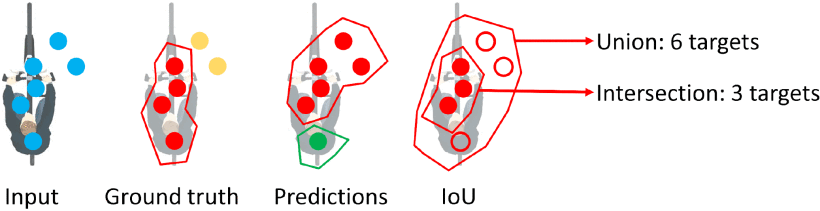
\includegraphics[width=0.95\linewidth]{images/iuo.png}
  \caption{Object-level metric. $Intersection / Union \geq 0.5$ counts as a true positive. In this example, there is a true positive cyclist and a false positive pedestrian detection.}
  \end{figure}
\end{itemize}

We selected Schumann {[}11{]} as a baseline because it is the only
multi-object, multi-class detection method found with small latency.
Also, \emph{Prophet} {[}1{]} is selected as a baseline. Since the DBSCAN
parameters are sensor-specific, the following table shows the optimal
parameters for the two baselines and for the class-specific clusters.
Both baselines method has the parameter \emph{v\textsubscript{min}},
used to find the static radar targets.

\begin{longtable}[]{@{}lllll@{}}
\toprule
\textbf{Method} & \textbf{$\mathbold{\gamma_{xy}}$} & \textbf{$\mathbold{  \gamma_v}$} &
\textbf{\emph{Min Points}} & \textbf{$\mathbold{ v_{  min}}$}\tabularnewline
\midrule
\endhead
\emph{Prophet} & 1.2 $m$ & 1.3 $m / s$ & 2 & 0.4
$m / s$\tabularnewline
\emph{Schumann} & 1.3 $m$ & 1.4 $m / s$ & 2 & 0.4
$m / s$\tabularnewline
Class specific: peds. & 0.5 $m$ & 2.0 $m / s$ & 1 & -\tabularnewline
Class specific: cyclists & 1.6 $m$ & 1.5 $m / s$ & 2 &
-\tabularnewline
Class specific: cars & 4.0 $m$ & 1.0 $m / s$ & 3 & -\tabularnewline
\bottomrule
\caption{Optimized DBSCAN parameters for the two baselines and the proposed method}
\end{longtable}

For two baselines, the classifiers consists of a Random Forest with 50
trees. The size of the cropped block are set to $L = W = 5, H = 32$.
The speed threshold to filter out static objects is a sensor-specific
parameter and was set to 0.3 \emph{m / s} based on empirical evidence.
The thresholds to merge clusters during object clustering were set to 1
$m$ spatially, 0.6 for scores, 2 $m / s$for pedestrian to cyclist,
and 1.2 $m / s$ for pedestrian/cyclist to car merges. The input data
are normalized to be zero-mean and have a standard deviation of 1.

\newpage
\subsection{Results}\label{header-n439}

\subsubsection{Experiments results}\label{header-n440}

The results of \emph{experiment 1} (target classification) are presented
in the following table.

\begin{longtable}[]{@{}llllll@{}}
\toprule
\textbf{Method} & \textbf{Pedestrian} & \textbf{Cyclist} & \textbf{Car}
& \textbf{Other} & \textbf{Avg}\tabularnewline
\midrule
\endhead
\emph{Prophet} & 0.61 & 0.58 & 0.34 & 0.91 & 0.61\tabularnewline
\emph{Schumann} & 0.67 & \textbf{0.68} & 0.46 & \textbf{0.92} &
0.68\tabularnewline
\emph{RTCnet (no low-level)} & 0.56 & 0.63 & 0.33 & 0.90 &
0.61\tabularnewline
\emph{RTCnet (no speed)} & 0.66 & 0.63 & 0.36 & 0.91 &
0.64\tabularnewline
\emph{RTCnet (no RCS)} & \textbf{0.71} & 0.66 & 0.48 & 0.91 &
0.69\tabularnewline
\emph{RTCnet (no ensemble)} & 0.67 & 0.65 & 0.47 & 0.89 &
0.67\tabularnewline
\emph{RTCnet} & \textbf{0.71} & 0.67 & \textbf{0.50} & \textbf{0.92} &
\textbf{0.70}\tabularnewline
\bottomrule
\caption{Target-wise scores divided per class obtained by the tested approaches}
\end{longtable}

\emph{RTCnet} outperformed the two cluster-wise baselines reaching an
average score of 0.70. \emph{Schumann} has slightly better results on
cyclists than \emph{RTCnet} (0.68 vs 0.67) but performs significantly
worse on pedestrians (0.67 vs 0.71) and cars (0.46. vs 0.50). The
ablation study showed that removing each feature yields worse results
than the complete pipeline, with the exception of \emph{RTCnet (no RCS)}
which has an average of 0.69. The results also show that classification
performance changes over the distance from the target object and the
vehicle, based on the number of samples in the training set. The figure
below shows this fact.

\begin{figure}[h!]
\centering
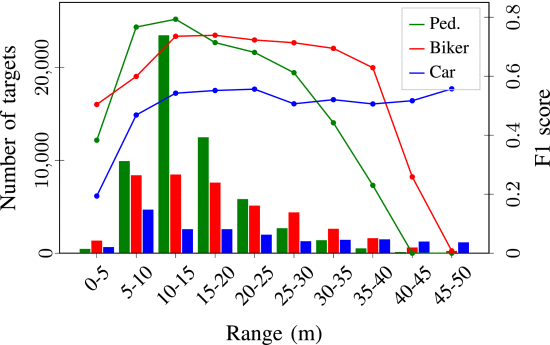
\includegraphics[width=0.85\linewidth]{images/resultsdistance.png}
\caption{Target-wise scores (lines) and number of targets in training set (bars) in function of distance from vehicle}
\end{figure}

For \emph{experiment 2} (object detection), the results are shown in the
following table.

\begin{longtable}[]{@{}lllll@{}}
\toprule
\textbf{Method} & \textbf{Pedestrian} & \textbf{Cyclist} & \textbf{Cars}
& \textbf{Avg.}\tabularnewline
\midrule
\endhead
\emph{Prophet} & 0.48 & 0.50 & 0.23 & 0.40\tabularnewline
\emph{Schumann} & 0.54 & \textbf{0.60} & 0.31 & 0.48\tabularnewline
\emph{RTCnet} & \textbf{0.61} & 0.59 & \textbf{0.47} &
\textbf{0.56}\tabularnewline
\bottomrule
\caption{Object-wise results obtained by the baselines and the proposed method}
\end{longtable}

\emph{RTCnet} reached slightly worse results on cyclists than
\emph{Schumann} (0.59 vs 0.60), but significantly outperformed it on
pedestrians (0.61 vs 0.54), cars (0.47 vs 0.31), and in average (0.56 vs
0.48).

\subsubsection{Discussion}\label{header-n528}

The proposed method outperformed the baselines in target classification
mainly due to two reasons. First, the classification does not depend on
a clustering step. This allows us to handle objects that contain a
single radar target (a common occurrence, especially for pedestrians)
and mitigates the difficult cases shows in the figure above. Second, the
method uses the low-level radar data, which brings the information of
the speed distribution around the radar target. To demonstrate that this
inclusion is beneficial, the authors show that only using target-level
data and only the third module of the network (\emph{RTCnet (no
low-level)}) caused a significant drop in performance from 0.70 to 0.61
average score. The results of RTCnet (no low-level) and RTCnet (no
speed) prove that the relative velocity distribution (i.e. the low-level
radar data) indeed contains valuable class information. Despite the
radar's performances are uniform in darkness/shadows/bright
environments, its typical errors are shown in the following figure.
Radar is easily reflected by flat surfaces (e.g. side of cars) acting
like mirrors, creating ghost targets.

\begin{figure}[h!]
\centering
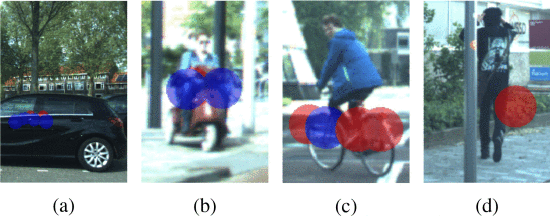
\includegraphics[width=0.85\linewidth]{images/rtcnetfails.png}
\caption{Examples of radar targets misclassified by RTCnet}
\end{figure}

The combination of the proposed network and the clustering step
outperformed the baseline methods in the object detection task. This is
mainly because by swapping the clustering and classifying steps, classes
can be clustered with different parameters. This is mainly because by
swapping the clustering and classifying steps, classes can be clustered
with different and more appropriate parameters.

\subsection{Conclusions}\label{header-n532}

In extensive experiments on a real-life dataset, the authors showed that
the proposed method improves upon the baselines in target-wise
classification by reaching an average score of 0.70 (vs. 0.68
\emph{Schumann}). Furthermore, the importance of low-level features and
ensembling in an ablation study is demonstrated. Furthermore, the
authors show that the proposed method outperforms the baselines overall
in object-wise classification by yielding an average score of 0.56 (vs.
0.48 \emph{Schumann}).
\newpage

\section{CorsNet: 3D Point Cloud Registration by Deep Neural
Network}\label{header-n534}

\emph{IEEE ROBOTICS AND AUTOMATION LETTERS, VOL. 5, NO. 3, JULY 2020}
{[}12{]}

\subsection{Introduction}\label{header-n536}

In computer vision, pattern recognition, and robotics, \emph{point set
registration}, also known as \emph{point cloud registration}, is the
process of finding a spatial transformation (\emph{e.g.,} scaling,
rotation and translation) that aligns two point clouds. The 3D point
cloud is a recently popular data format. The most popular and classic
method for point cloud registration is the iterative closest point (ICP)
algorithm {[}13{]}. ICP calculates the rigid motion based on a fixed
correspondence between one point cloud and another, updating the
correspondence to minimize the point-to-point distances. Although ICP
can achieve highly accurate registration, the registration often fails
by falling into the local minimum. In other words, the registration
accuracy of ICP depends strongly on its initial perturbation. Despite
this, the inherent lack of structure has caused difficulties when
adopting point clouds as direct input in deep learning architecture.
PointNet {[}14{]}, overcomes these difficulties, providing a mechanism
to extract the feature related to the point clouds. PointNet is a
general representation of an unstructured point cloud that allows object
detection, segmentation, and so on. PointNetLK {[}15{]} is the latest
deep learning-based registration techniques using PointNet {[}2{]}.
PointNetLK directly optimizes the distance of aggregated features using
the gradient method. This approach overcomes computational speed and
local minimum problems. In this paper, ``DirectNet" is proposed as a
baseline method as it is a simplistic approach. However, the authors
think that PointNetLK and DirectNet do not consider local features,
falling to fully utilize the point cloud information. In this work,
CorrespondenceNet (CorsNet) is proposed. It is a novel point cloud
registration method based on deep learning is proposed. This method
feeds global features from PointNet to per-point local features to make
effective use of point cloud information. The end-to-end network
architecture consists of the main three parts: (1) extracting global
features of point clouds with PointNet, (2) concatenating global
features with local features of the source point cloud and outputting
the correspondences of each point via fully connected layers and (3)
estimating a rigid transform with singular value decomposition (SVD).
The SVD part is also included in the end-to-end network architecture.
The singular value decomposition is a factorization of a matrix
$m \times n$. Given the matrix here $\mathbf {M}_{m\times n}$,
$\mathbf{M} = \mathbf{U}\mathbf{\Sigma}\mathbf{V}$. If $\mathbf {M}$ is used
in a geometrical operation, the same result can be obtained applying
these three matrices in succession. In particular,
$\mathbf {U}_{m\times n}$ is an orthogonal matrix that applies a
rotation, $\mathbf{\Sigma}_{n\times n}$ is a diagonal matrix that scales only
the axes and $\mathbf {V}_{n\times q}$ is another orthogonal matrix
that applies another rotation.
\newpage
\begin{figure}[h!]
\centering
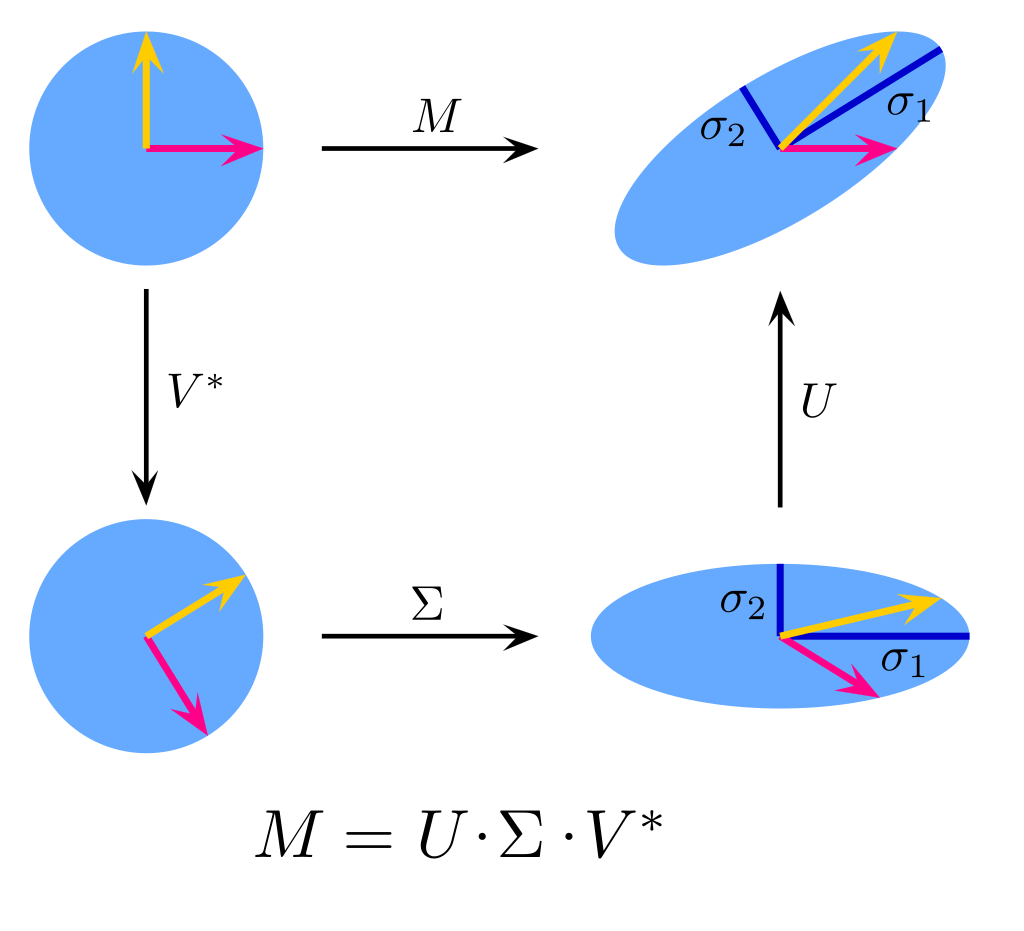
\includegraphics[width=0.7\linewidth]{images/singolarvaluedec.png}
\caption{Singular value decomposition}
\end{figure}

\subsection{Proposed method (CorsNet)}\label{header-n539}

A point cloud is represented as a set of 3D points
$\{P : P_i|i = 1, . . ., n\} \subset \R_3$ whose each point $P_i$ is
a vector of its $(x, y, z)$ coordinate. The following figure shows the
CorstNet architecture.

\begin{figure}[h!]
\centering
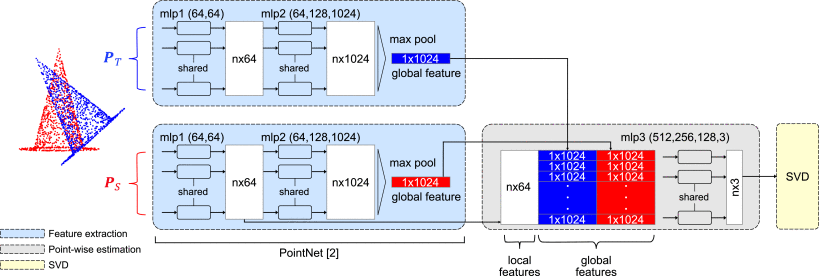
\includegraphics[width=0.8\linewidth]{images/corsnetarch.png}
\caption{CorsNet architecture}
\end{figure}

The red $\boldsymbol{P}_S$ and blue $\boldsymbol{P}_T$ point clouds
represent the \emph{source} and \emph{template} point clouds,
respectively. We find the rigid transform $\boldsymbol{G} \in SE$,
which includes the alignment between $\boldsymbol{P}_S$ and
$\boldsymbol{P}_T$. The model mainly consists of three components:

\begin{itemize}
\item
  \textbf{Global feature extraction:} this first module extract the
  point cloud's features. These features must include three factors:
  invariance in order, acquisition of local feature, and invariance in
  rotation. PointNet is used to absolve this goal. It satisfying these
  three requirements and it has achieved high accuracy and low
  computational complexity in various benchmarks. The PointNet output is
  a $1 \times 1024$ vector obtained by a max-pooling of two MLP (multi-layer
  perceptron). The features are extracted both for the source and
  template point clouds.
\item
  \textbf{Correspondence estimation:} after computing the global
  features of the source and template point cloud, this module finds the
  point local features by concatenating the global feature with each of
  the point features. The network output is t
  $\Delta\boldsymbol{P}_S$, a $n \times 3$ matrix. By adding this
  $\Delta\boldsymbol{P}_S$ to $\boldsymbol{P}_S$, the tentative
  transform destination can be calculated as follow:

  $ \hat{\boldsymbol {P}_T} = \boldsymbol {P}_S + \Delta \boldsymbol {P}_S $

  This method regresses correspondences $\Delta\boldsymbol{P}_S$ and
  estimates a rigid transform based on the estimated correspondences
  using SVD

  $ \boldsymbol {G}\cdot \boldsymbol {P}_S= \boldsymbol {P}_T$
\item
  \textbf{SVD:} the source point cloud is now aligned with the template
  point cloud and the following is the approach for calculating a rigid
  transformation using SVD as follows.

  Define the centroids of $\boldsymbol{P}_S$ and
  $\hat{\boldsymbol{P}_T}$ as:

  $\overline{\boldsymbol {P}_S} = \frac{1}{n}\sum ^{n}_{i=1}\boldsymbol {P}_S \;\;\; \text{and} \;\;\; \overline{\hat{\boldsymbol {P}_T}} = \frac{1}{n}\sum ^{n}_{i=1}\hat{\boldsymbol {P}_T}$

  and calculate the cross-covariance matrix H:

  $ \boldsymbol {H}= \sum ^{N}_{i=1}\left(\hat{\boldsymbol {P}_T}-\overline{\hat{\boldsymbol {P}_T}}\right)\left(\boldsymbol {P}_S-\overline{\boldsymbol {P}_S}\right)^{T}.$

  Then, use SVD to decompose $\boldsymbol{H}$ to
  $\boldsymbol{U},\boldsymbol{V} \in SO$

  $  [\boldsymbol {U}, \boldsymbol {S}, \boldsymbol {V}]= SVD (\boldsymbol {H}).$

  and, using this decomposition, extract the rigid transform elements,
  estimated rotation, $\boldsymbol{R}_{est}\in SO$ and translation,
  $\boldsymbol{t}_{est} \in \R^3$

  $ \boldsymbol {R}_{est} = \boldsymbol {V}\boldsymbol {U}^{T}.\\\boldsymbol {t}_{est} = - \boldsymbol {R}\cdot \overline{\hat{\boldsymbol {P}_T}} + \overline{\boldsymbol {P}_S}. $

  Now, it is possible to calculate the estimated rigid transform
  $\mathbf{G}_{est}$ and the twist parameters
  $\mathbf{\xi}_{est} \in \R^{6}$ as follow:

  $ \boldsymbol {G}_{est} = \left(\begin{array}{cc}\boldsymbol {R}_{est} & \boldsymbol {t}_{est} \\ \boldsymbol {0} & 1 \end{array} \right). \\ \boldsymbol {\xi }_{est} = \phi \left(\boldsymbol {G}_{est} \right). $
\end{itemize}

\newpage
The dataset used to test the proposed method is called ModelNet40
{[}16{]}. From this, the source point clouds ($\boldsymbol{P}_S$) are
extracted and the ground-truth estimated rigid transform
($\boldsymbol{G}_{gt}$) can be defined as:\newline\
$ \boldsymbol {P}_{T} = \boldsymbol {G}_{gt}\cdot \boldsymbol {P}_{S}.$\newline
Now, we call $\boldsymbol{Cors}$ the correspondence between two point
clouds, in particular: \newline
$\boldsymbol {Cors}_{gt} = \boldsymbol {P}_{T} - \boldsymbol {P}_{S}.  \\  \boldsymbol {Cors}_{est} = \hat{\boldsymbol {P}_{T}} - \boldsymbol {P}_{S}.$
\newline
Subsequently, we define three kinds of loss elements using previously
values:
\newline
$ \boldsymbol {loss}_{1} = ||(\boldsymbol {G}_{est})^{-1}\cdot \boldsymbol {G}_{gt} - \boldsymbol {I}_{4}||_{F}. \\ \boldsymbol {loss}_{2} = ||\boldsymbol {\xi }_{gt}-\boldsymbol {\xi }_{est}||^{2}. \\ \boldsymbol {loss}_{3} = ||\boldsymbol {Cors}_{gt} - \boldsymbol {Cors}_{est}||^{2}. $
\newline
From them, four loss functions are defined as follow:
\newline
$ \boldsymbol {Loss}_{v1} = \boldsymbol {loss}_{1}. \\ \boldsymbol {Loss}_{v2} = \boldsymbol {loss}_{2}. \\ \boldsymbol {Loss}_{v3} = \boldsymbol {loss}_{1} + \boldsymbol {loss}_{3}.\\ \boldsymbol {Loss}_{v4} = \boldsymbol {loss}_{2} + \boldsymbol {loss}_{3}.  $
\newline
The authors verified the effectiveness of each loss function in the
experiments.

\subsection{Proposed method (DirectNet)}\label{header-n572}

The authors proposed a novel method which directly regresses the pose,
including rotation $\boldsymbol{R}_{euler} \in \R^3 $ (Euler angle) and
translation $\boldsymbol{t} \in \R^3$, as shown in the following figure.

\begin{figure}[h!]
\centering
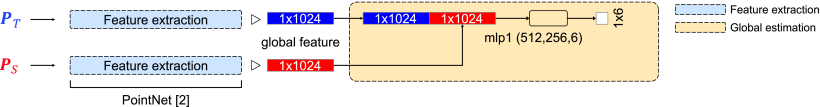
\includegraphics[width=0.95\linewidth]{images/directnet.png}
\caption{DirectNet architecture}
\end{figure}

DirectNet consists of two parts: the global feature extraction module,
which is identical to CorsNet (that is PointNet), and the global
estimation part. The $\boldsymbol{P}_S$ and $\boldsymbol{P}_T$
global features extracted with PointNet are concatenated and converted
to $1 \times 6$ vector. The output $1 \times 6$ vectors is
$[x_{euler}, y_{euler}, z_{euler}, x_{t}, y_{t}, z_{t}]^T$. The first
half of this vector is represented as
$\boldsymbol{R_{euler}} = [x_{euler}, y_{euler}, z_{euler}]^T$ . This
$\boldsymbol{R_{euler}}$ is converted into
$\boldsymbol{R_{est}} \in SO $ as follows:
\newline
$ \boldsymbol {x}_{mat} = \left(\begin{array}{ccc}1 & 0 & 0 \\ 0 & \cos x_{euler} & -\sin x_{euler} \\ 0 & \sin x_{euler} & \cos x_{euler} \end{array} \right), \\ \boldsymbol {y}_{mat} = \left(\begin{array}{ccc}\cos y_{euler} & 0 & \sin y_{euler} \\ 0 & 1 & 0 \\ -\sin y_{euler} & 0 & \cos y_{euler} \end{array} \right), \\ \boldsymbol {z}_{mat} = \left(\begin{array}{ccc}\cos z_{euler} & -\sin z_{euler} & 0 \\ \sin z_{euler} & \cos z_{euler} & 0 \\ 0 & 0 & 1 \end{array} \right), \\ \boldsymbol {R}_{est} = \boldsymbol {x}_{mat} \cdot \boldsymbol {y}_{mat} \cdot \boldsymbol {z}_{mat} $ 
\newline
The last part, instead, define the translation vector
$\boldsymbol{t_{est}}$ as
\newline
$ \boldsymbol {t}_{est} = [x_{t}, y_{t}, z_{t}]^{T}.$
\newline
Using $\boldsymbol {R}_{est}$ and $\boldsymbol {t}_{est}$ is
possible to determine $\boldsymbol {G}_{est}$ and
$\boldsymbol {\xi}_{est}$ as done for CorsNet. For DirectNet two loss
functions are formulated:
\newline
$ \boldsymbol {Loss}_{v1} = ||(\boldsymbol {G}_{est})^{-1}\cdot \boldsymbol {G}_{gt} - \boldsymbol {I}_{4}||_{F}. \\ \boldsymbol {Loss}_{v2} = ||\boldsymbol {\xi }_{gt}-\boldsymbol {\xi }_{est}||^{2}.$

\subsection{Experiments}\label{header-n581}

The proposed method CorsNet is compared with ICP and PointNetLK,
DirectNet (described in this work). The figure below shows graphical examples of pointcloud registration, each of them is executed with a different approach.

\begin{figure}[h!]
\centering
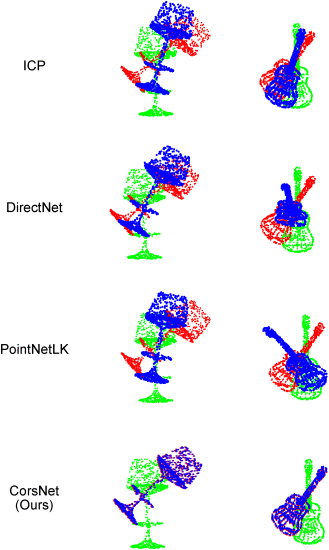
\includegraphics[width=0.4\linewidth]{images/pointcloudreg.png}
\caption{Point cloud registration. \emph{Green}: source, \emph{Blue}: template, \emph{Red}: transformed point cloud. Only the proposed method achieves accurate registration regardless of the initial perturbations.}
\end{figure}

The dataset used is ModelNet40, which includes various point clouds with
40 categories. The point clouds' coordinates are normalized to be in the
$[0, 1]^3$ interval and the points of each model's surface are
sampling to be exactly 1024. The authors measure the root mean square
error (RMSE) of rotation $\boldsymbol{R}$ and translation
$\boldsymbol{t}$ for each experimental setting. The first experiment
consists into evaluate the models using the same categories. 20
categories from the dataset were chosen and they are used for both
training and testing of all networks. CorsNet and DirectNet were trained
using all the losses reported in the sections above. The authors chose a
ground-truth transformation ($\boldsymbol{G}_{gt}$) randomly by an
interval of $[0, 45]$ degrees for rotation and $[0, 0.8]$ for
translation. The following table shows the evaluation results of all
models, using all possible loss functions.

\begin{longtable}[]{@{}lll@{}}
\toprule
\textbf{Method (loss type)} & \textbf{RMSE ($\boldsymbol{R}$)} &
\textbf{RMSE ($\boldsymbol{t}$)}\tabularnewline
\midrule
\endhead
ICP & 46.4628 & 0.26144\tabularnewline
DirectNet $\boldsymbol{Loss}_{v1}$ & 19.4791 & 0.01218\tabularnewline
DirectNet $\boldsymbol{Loss}_{v2}$ & 20.9916 & 0.01690\tabularnewline
PointNetLK & \textbf{14.9746} & 0.01690\tabularnewline
CorsNet $\boldsymbol{Loss}_{v1}$ & 18.6482 & 0.01574\tabularnewline
CorsNet $\boldsymbol{Loss}_{v2}$ & 17.9941 & 0.00725\tabularnewline
CorsNet $\boldsymbol{Loss}_{v3}$ & 18.8303 &
\textbf{0.00632}\tabularnewline
CorsNet $\boldsymbol{Loss}_{v4}$ & 16.2356 & 0.00693\tabularnewline
\bottomrule
\caption{Comparison results on same categories}
\end{longtable}

The results show that the proposed CorsNet, whose loss function is
$\boldsymbol{Loss}_{v3}$, achieved the highest accuracy in terms of
translation. The following figure shows (on its left part) the ratio
between the root mean square error with respect to perturbation both for
rotation and translation. To verify the robustness of the categories,
the authors evaluated the proposed network architecture using different
categories for training and testing. This is the second experiment. The
table below reports the performance evaluation results for the proposed
and related methods.

\begin{longtable}[]{@{}lll@{}}
\toprule
\textbf{Method (loss type)} & \textbf{RMSE ($\boldsymbol{R}$)} &
\textbf{RMSE ($\boldsymbol{t}$)}\tabularnewline
\midrule
\endhead
ICP & 45.8016 & 0.28369\tabularnewline
DirectNet $\boldsymbol{Loss}_{v1}$ & 20.8310 & 0.01983\tabularnewline
DirectNet $\boldsymbol{Loss}_{v2}$ & 22.0024 & 0.01712\tabularnewline
PointNetLK & 21.0866 & 0.03525\tabularnewline
CorsNet $\boldsymbol{Loss}_{v1}$ & 20.2198 & 0.02401\tabularnewline
CorsNet $\boldsymbol{Loss}_{v2}$ & 20.3712 & 0.02396\tabularnewline
CorsNet $\boldsymbol{Loss}_{v3}$ & 19.4610 & 0.02288\tabularnewline
CorsNet $\boldsymbol{Loss}_{v4}$ & \textbf{16.7927} &
\textbf{0.01398}\tabularnewline
\bottomrule
\caption{Comparison results on different categories}
\end{longtable}

Rotation and translation are estimated most accurately by CorsNet, whose
loss function is $\boldsymbol{Loss}_{v4}$. The following figure shows
(on its right part) the ratio between the root mean square error with
respect to perturbation both for rotation and translation.

\begin{figure}[h!]
\centering
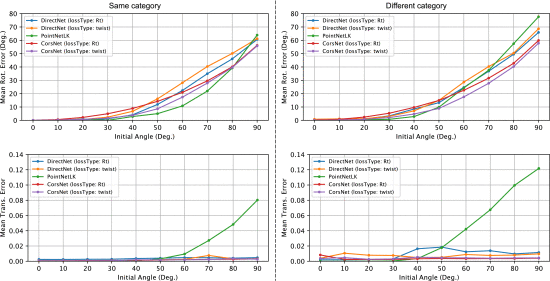
\includegraphics[width=0.95\linewidth]{images/mod.png}
\caption{Each graph shows the transition of a root mean square error with respect to the initial perturbation (rotation and translation). The left part refers to the experiments on the same category while the right part refers different categories' experiments}
\end{figure}

\subsection{Conclusions}\label{header-n662}

The superiority of the proposed method has been proven qualitatively and
quantitatively. CorsNet $\boldsymbol{Loss}_{v3}$ and CorsNet
$\boldsymbol{Loss}_{v4}$ ware appreciably more accurate thanCorsNet
$\boldsymbol{Loss}_{v1}$ and CorsNet $\boldsymbol{Loss}_{v2}$,
depending on whether the correspondence loss is included in the loss
function. The following two figure shows the registration results for
the methods tested. Only the proposed method (CorsNet) successfully
aligns the point clouds without falling into the local minimum,
especially where the input point clouds include the repeating
structures.

\begin{figure}[h!]
\centering
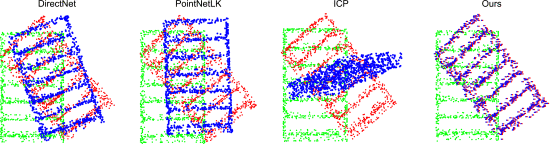
\includegraphics[width=0.95\linewidth]{images/registrationres.png}
\caption{Comparison with DirectNet, PointNetLK, and ICP (green: source, blue: template, red: transformed)}
\end{figure}

The authors suppose that this is because only the proposed method links
the local features to the global features, making the most of the local
and global point cloud information.
\newpage

\section{Learning Deep NBNN Representations for Robust Place
Categorization}\label{header-n666}

\emph{IEEE ROBOTICS AND AUTOMATION LETTERS, VOL. 2, NO. 3, JULY 2017}
{[}17{]}

\subsection{Introduction}\label{header-n668}

An important aspect of human-robot interaction is the ability of
artificial agents to understand the way humans think and talk about
abstract spatial concepts. To do this, an autonomous agent has to
extract information from its sensor to assign a semantic labels to a
specific place. In particular, this work focuses on assign label to
images. The most important challenges in identifying places come from
the complexity of the concepts to be recognized and from the variability
of the conditions in which the images are captured. In fact, scenes from
the same category may differ significantly, while images corresponding
to different places may look similar. The historical take on these
issues has been to model the visual appearance of scenes considering a
large variety of (shallow) learning models (e.g. SVMs, Random Forests),
but approaches based on learning deep representations have become
mainstream. Some work, like {[}19{]}, demonstrated the benefits derived
from feature extraction through convolutional deep neural networks.
Subsequent studies demonstrated the benefits of region-based approaches
(i.e. considering only specific image parts) in combination with
descriptors derived from CNNs, such as to obtain models that are robust
to viewpoint changes and occlusions. Other successful works tried to
bring back the notion of localities into deep networks, e.g. by
designing appropriate pooling strategies or by casting the problem
within the Image-2-Class (I2C) recognition statements, with a high
degree of success. Despite this, these methods implement the CNN feature
extraction and the classifier learning as two separate modules. This
leads to two drawbacks: first, choosing heuristically the relevant
localities means concretely cropping parts of the images before feeding
them to the chosen features extractor. Second, it would be desirable to
fully exploit the power of deep networks by directly learning the best
representations for the task at hand, rather than re-use architectures
trained on general-purpose databases like ImageNet. This work proposes
an approach for semantic place categorization which exploits local
representations within a deep learning framework. The method is inspired
by the recent work {[}18{]}, which demonstrates that, by dividing images
into regions and representing them with CNN-based features,
state-of-the-art scene recognition accuracy can be achieved by
exploiting an I2C approach, namely a parametric extension of the Naıve
Bayes Nearest Neighbor (NBNN) model. The deep architecture for semantic
scene classification seamlessly integrates the NBNN and CNN frameworks.
We automatize the multi-scale patch extraction process by adopting a
fully-convolutional network, guaranteeing a significant advantage in
terms of computational cost over two-steps methods. This is the first
attempt to fully unify NBNN and CNN, building a network in which the
NBNN error is back-propagated to the CNN in a unified end-to-end
training.

\begin{figure}[h!]
\centering
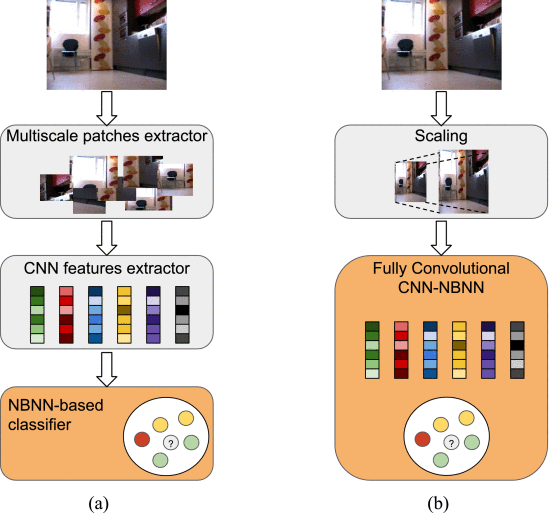
\includegraphics[width=0.6\linewidth]{images/NBNNdiff.png}
\caption{The standard NBNN classification pipeline (a) versus the proposed model (b)}
\end{figure}

\subsection{Proposed method}\label{header-n671}

As represented in the figure above, images are decomposed into multiple
regions (represented with CNN features) and a part-based classifier is
used to infer the labels associated with places. However, differently
from previous works, the proposed approach unifies the feature
extraction and the classifier learning phases. Since this framework is
derived from previous NBNN-based works, it is important to give an
overview of this method.

\subsubsection{Naıve Bayes Non-Linear Learning }\label{header-n673}

Let ${\mathcal X}$ denote the set of possible images and let
${\mathcal Y}$ be a finite set of class labels, indicating the
different scene categories. The goal is to estimate a classifier
$f : {\mathcal X} \rightarrow {\mathcal Y}$ from a training set
${\mathcal T} \subset {\mathcal X} \times {\mathcal Y}$. The NBNN
method works under the assumption that there is an intermediate
Euclidean space $Z$ and a set-valued function $\phi$ that abstracts
an input image $x \in {\mathcal X}$ into a set of descriptors in
${\mathcal Z}$, i.e. $\phi(x) \subset {\mathcal Z}$. For instance,
the image could be broken into patches and a descriptor in
${\mathcal Z}$ could be computed for each patch. Given a training set
${\mathcal T}$, let $\Phi_y({\mathcal T})$ be the set of descriptors
computed from images in ${\mathcal T}$ having labels
$y \in {\mathcal Y}$, i.e.
$\Phi_y({\mathcal T}) = \{\phi(x): x \in {\mathcal X}, (x, y) \in {\mathcal T}\}$
. The NBNN classifier $f_{NBNN}$ is given as follows:
\newline
$ f_\mathtt {NBNN}(x; {\mathcal T})=\text{arg min}_{y\in {\mathcal Y}}\sum _{z\in \phi (x)}d(z,\Phi _y({\mathcal T}))^2\,, $
\newline
where $d(x, {\mathcal S}) = \inf\{\| z − s\|_2 : s \in {\mathcal S}\}$
denotes the smallest Euclidean distance between $z$ and an element of
$  {\mathcal S} \subset {\mathcal Z}$. $f_{NBNN}$ has the drawback
of being expensive at test time, due to the nearest-neighbor search. A
possible way to reduce the complexity consists of learning a small,
finite set ${\mathcal W}_y \subset {\mathcal Z}$ of representative
prototypes for each class $y \in {\mathcal Y}$ to replace
$\Phi_y({\mathcal T})$. This idea generates NBNL (Naıve Bayes
Non-Linear Learning). NBNL is developed by replacing
$\Phi_y({\mathcal T})$ with the set of prototypes ${\mathcal W}_y$
and by assuming ${\mathcal Z}$ to be restricted to the unit ball.
Under the latter assumption the bound
$d(z, {\mathcal S})^{2} = 2 - \omega(z, {\mathcal S}) $ can be
derived, where
\newline
$ \omega (z, {\mathcal S})= \left(\sum _{s\in {\mathcal S}}|\langle z,s\rangle |_+^{q}\right)^{1/q}\,. $
\newline
Here, $\langle \cdot \rangle$ denotes the dot product,
$q \in [1, +\infty]$ and $[x]_+ = \max(0, x)$. Finally, the NBNL is
defined as follows (substituting $d()^{2}$)
\newline
$ f_\mathtt {NBNL}(x; {\mathcal W})=\text{arg max}_{y\in {\mathcal Y}}\sum _{z\in \phi (x)}\omega (z, {\mathcal W} _y)\,. $
\newline
In order to learn the prototypes ${\mathcal W}_y$ for each
$y \in {\mathcal Y}$, each descriptor extracted from an image is
promoted to a training sample.

\subsubsection{CNN-NBNL}\label{header-n681}

The NBNL model is subsequently combined with a CNN, capable of
extracting images' descriptors. In this method, called CNN-NBNL,
$\phi(x)$ (the function which extracts descriptors form any image
$x \in {\mathcal X}$) is obtained by dividing an image into patches at
different scales and by employing a pre-trained CNN-based feature
extractor. Formally, if
$g_{CNN} : {\mathcal X} \rightarrow {\mathcal Z}$ is the CNN-based
feature extractor, $\phi(x)$ is define as follows:
\newline
$ \phi _\mathtt {CNN}(x)=\lbrace g_\mathtt {CNN}(\hat{x})\,:\,\hat{x}\in \text{patches}(x)\rbrace \,, $
\newline
where $patches(x) \subset {\mathcal X}$ returns a set of patches
extracted from the image $x$ at multiple scales (${\hat x}$ is a
scaled image), $g_{CNN}$ is a CNN implementation and
$g_{CNN}({\hat x})$ is a single descriptor obtained by the image
${\hat x}$. At test time, $f_{NBNL}$ is used with $\phi$ replaced
by $\phi_{CNN}$. By moving from hand-crafted features to CNN-based
features, the performance of the NBNL classifier improves considerably.
Nonetheless, this approach has two limitations:

\begin{itemize}
\item
  it requires the extraction of patches for each image as a
  pre-processing step and
\item
  the CNN architecture is used as a mere feature extractor and the
  method lacks the advantage of an end-to-end trainable system.
\end{itemize}

\subsubsection{Fully-convolutional CNN-NBNL}\label{header-n690}

To overcome the two limitations reported in the above section, the
method proposed in this work uses a fully-convolutional network that
incorporates both the CNN features extractor and the NBNL algorithm,
making them trainable together. First of all, this model resolves the
problem of extracting patches. In fact, this operation, and the
subsequent feature extraction performed by CNN, is highly
time-consuming. To do this faster, the CNN is replaced by a
Fully-Convolutional CNN (FC-CNN), derived from a standard CNN by
replacing fully-connected layers with convolutional layers. This network
maps an input image of arbitrary size into a set of spatially-arranged
output values (descriptors). To simulate multiple scales, the FC-CNN
analyzes images from different resolutions, forcing an implicit change
of scale in the final descriptors. The FC-CNN is formally called
$g_{FCN}$. Its outputs, defined as$g_{FCN}(x, \theta)$ ($\theta$
are the network parameters), is a set of descriptors, one for each
spatial location of the final convolutional layer. Defined the FC-CNN
that extracts the images' descriptors, the attention is placed on the
NBNL classifier. It can be implemented using layers that are commonly
found in deep learning frameworks and can thus be easily stacked on top
of an FC-CNN. By doing so, the architecture obtained can be trained in
an end-to-end way. The final form of the NBNL classifier is given by:
\newline
$ f_\mathtt {FCN\,NBNL}(x; {\mathcal W},\theta)=\text{arg max}_{y\in {\mathcal Y}}h(x; {\mathcal W} _y,\theta)\,, $
\newline
where $h$ defined below measures the likelihood of $x$ given
prototypes in ${\mathcal W}_y$:
\newline
$ h(x; {\mathcal W} _y,\theta)=\frac{1}{m}\sum _{\hat{x}\in \text{scale(x)}}\bar{\omega }(\hat{x}; {\mathcal W} _y,\theta) $
\newline
and $\bar \omega$ is is the scale-specific normalized score:
\newline
$ \bar{\omega }(\hat{x}; {\mathcal W} _y,\theta)=\frac{1}{\eta (\hat{x})}\sum _{z\in g_\mathtt {FCN}(\hat{x};\theta)}\omega (z; {\mathcal W} _y)\,. $
\newline
where $\eta(x)$ is the number of descriptors generated by the FC-CNN
from the image $x$. The following figure describes the architecture of
the entire system, with particular attention to the NBNL module. The
scaled versions of an image $x$, defined as
$\{\hat x_1, ...., \hat x_m\} = scale (x)$, are forwarded in parallel
through the net. The green block represents the FC-CNN, while the gray
ones implement the NBNL classifier. The red blocks, instead, are active
only during training. Parameter $k$ represents the number of classes,
$p$ the number of prototypes per class and $q$ is the parameter of
the Naıve Bayes Non-Linear Learning algorithm. $conv[W,C]$ is a
$W \times W$ convolutional layer with $C$ filters. $relu$ applies
the ReLu non-linearity to each element. $pow[E] $ raises each element
to the power of $E$. $gconv[G,W,C]$ is a grouped $W \times W$
convolutional layer with $G$ groups and $C$ filters. $reduce[avg]$
averages out the spatial dimensions. $sum$ performs the element-wise
sum of the incoming lines. $argmax$ returns the index of the maximum
element. $softmax$ applies the softmax operator (normalizes vector
values to be in the {[}0, 1{]} range with a sum of 1) along the input
channels, for each spatial entry of each input line.
$logloss[ \frac{1}{\eta (\hat{x}_i)} ]$ sums up the log-loss computed
along the input channels of each spatial entry of each input line, and
each input line is weighted by $\frac{1}{\eta (\hat{x}_i)}$ .

\begin{figure}[h!]
\centering
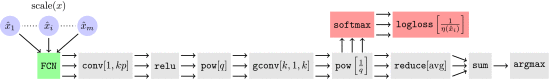
\includegraphics[width=0.95\linewidth]{images/CNNNBNL.png}
\caption{The architecture of the proposed method, fully convolutional CNN-NBNL}
\end{figure}

\subsection{Experimental results}\label{header-n699}

\subsubsection{Proposed method comparison with
baselines}\label{header-n700}

In the first series of experiments, the proposed method is compared with
its non-end-to-end counterpart: a CNN-NBNL approach explained in
{[}18{]}. In addition, other two holistic approaches are chosen for
testing the FC-CNN-NBNL method. Both of them have been proposed by Zhou
\emph{et al.} {[}23{]}, {[}24{]}, in which they pre-train a CNN with a
huge dataset and use it as features extractor for learning a linear SVM
model. To demonstrate the generality of this work, all approaches are
tested through three different base networks: the Caffe {[}20{]} version
of AlexNet {[}19{]}, VGG-16 {[}21{]} and GoogLeNet {[}22{]}. To decide
the proper learning rate schedule and number of epochs, the authors
performed parameters tuning on a separate validation set. As parameters
of the NBNL classifier, the authors chose $k = 10$ and $p = 2$,
applying a weight decay of $10^{-5}$ on the prototypes. Notice that
the model proposed in this work considered 110 descriptors, while 100
were used for the baseline method in {[}13{]}. However, it has been
experimentally verified that a difference of 10 descriptors does not
influence performance. The experiments are performed using three
different datasets: Sports8 (which contains 8 different indoor and
outdoor sport scenes), Scene15 (composed by different categories of
outdoor and indoor scenes) and MIT67 (which contains images of 67 indoor
scenes). For each dataset, the authors took 5 random splits, reporting
the results as mean and standard deviation. The following table shows
the results of this evaluation.

\begin{longtable}[]{@{}lllll@{}}
\toprule
\textbf{Network} & \textbf{Method} & \textbf{Sport8} & \textbf{Scene15}
& \textbf{MIT67}\tabularnewline
\midrule
\endhead
& {[}23{]} & $94.22\pm0.78$ & $91.59\pm0.48$ & 70.8\tabularnewline
AlexNet & {[}18{]} & $95.29 \pm 0.61$ & $92.42 \pm 0.64$ & $73 \pm
0.36$\tabularnewline
& FC-CNN-NBNL & $\boldsymbol{95.58 \pm 0.58}$ & $\boldsymbol{93.63 \pm 0.90}$ &
$\boldsymbol{74.98 \pm 0.78}$\tabularnewline
& {[}24{]} & $91.00$ & 91.25 & 73.30\tabularnewline
GoogLeNet & {[}18{]} & $93.08 \pm 1.78$ & $92.29 \pm 0.59$ & $73.14 \pm
1.43$\tabularnewline
& FC-CNN-NBNL & $\boldsymbol{94.46 \pm 0.86}$ & $\boldsymbol{93.68 \pm 0.57}$ &
$\boldsymbol{80.55 \pm 0.70}$\tabularnewline
& {[}24{]} & 94.17 & 92.12 & 77.63\tabularnewline
VGG-16 & {[}18{]} & $94.79 \pm 0.42$ & $92.97 \pm 0.68$ & $77.62 \pm
0.97$\tabularnewline
& FC-CNN-NBNL & $\boldsymbol{97.04 \pm 0.27}$ & $\boldsymbol{95.12 \pm 0.41}$ &
$\boldsymbol{82.49 \pm 1.35}$\tabularnewline
\bottomrule
\caption{Comparing global and part based CNN models}
\end{longtable}

Mean and standard deviation are provided for FC-CNN-NBNL and {[}13{]}
methods, while for the CNN models in {[}30{]}, {[}31{]} the authors
report results from the original letters. For all base networks and
datasets, the proposed method outperforms the baselines. Moreover, the
end-to-end training model guarantees an improvement in performance
compared to its non-end-to-end counterpart CNN-NBNL. While a pre-trained
CNN isn't able to extract discriminative features when applied to a
specific task, end-to-end training allows to adapting the trained
features to fit a precise task. The figure below shows the difference in
expressivity form feature extracted by {[}18{]} and the proposed method.

\begin{figure}[h!]
\centering
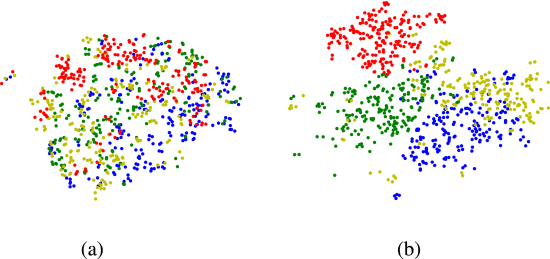
\includegraphics[width=0.8\linewidth]{images/tsneNBNL.png}
\caption{t-SNE visualization of features extracted from 4 classes of the Scene15 dataset: (a) [18], (b) FC-CNN-NBNL}
\end{figure}

To further compare our approach and CNN-NBNL {[}18{]}, the authors also
analyzed the computational time required during the test phase to
process an increasing number of patches. The following figure reports
the results of this analysis: as expected, the fully-convolutional
architecture is greatly advantageous over the CNN-NBNL.

\begin{figure}[h!]
\centering
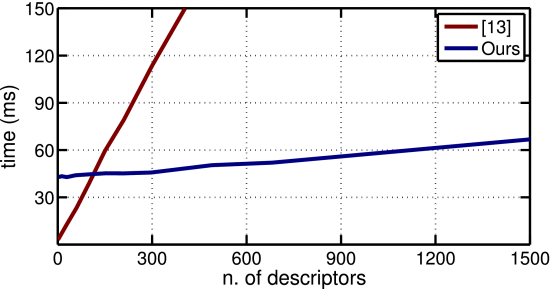
\includegraphics[width=0.7\linewidth]{images/NBNLtime.png}
\caption{Computational time at varying number of descriptors}
\end{figure}

\subsubsection{Proposed method performance in robot place
categorization}\label{header-n767}

These experiments aim to test the proposed method on available robot
datasets, in order to verify its robustness to varying environmental
conditions and occlusions.

The first tested dataset is called \emph{COsy Localization Database}
(COLD). This database contains three datasets of indoor scenes acquired
in three different laboratories from different robots: COLD-Freiburg,
COLD-Ljubljana and COLD-Saarbrucken. These data depict significant
changes with respect to illumination conditions and time of data
acquisition. The models are trained and tested on data collected in the
same laboratory, considering 5 random splits and reporting the average
values. The following table shows the comparison between the CNN
approach explained in {[}23{]} and the proposed method.

\begin{longtable}[]{@{}llll@{}}
\toprule
\textbf{Method} & \textbf{Freiburg} & \textbf{Saarbrcken} &
\textbf{Ljubljana}\tabularnewline
\midrule
\endhead
{[}23{]} & \textbf{96.1} & 96.8 & 98.6\tabularnewline
FC-CNN-NBNL & 95.2 & \textbf{97.3} & \textbf{99.2}\tabularnewline
\bottomrule
\caption{Results on COLD dataset}
\end{longtable}

Despite the {[}23{]} method outperforms the proposed method for
COLD-Freigurg dataset, the high accuracy of our method also demonstrates
that FC-CNN-NBNL is highly effective at discerning among different
rooms, even with significant lighting and environmental changes.

The second dataset used for testing the model proposed is called
\emph{KTH Image Database for rObot Localization} (KTH-IDOL). This
dataset contains image sequences collected by two robots (Dumbo and
Minnie) on 5 different rooms along several days on three different
illumination conditions: sunny, cloudy and night. Using this dataset,
three different types of tests are performed. First, the authors trained
and tested using the same robot and the same weather conditions with one
sequence used for training and another for testing and vice-versa. As a
second experiment, the authors used the same robot for training and
testing, varying the weather conditions of the two sets. In the last
experiment, the classifier is trained with the same weather condition
but it is tested on a different robot. The model proposed in this work
is compared with {[}23{]} and three state-of-the-art approaches:

\begin{itemize}
\item
  {[}25{]} which used high dimensional histogram global features as
  input for a ${\mathcal X}^{2}$ kernel SVM; 
\item
  {[}24{]} which proposed the CENTRIST descriptor and performed nearest
  neighbor classification;
\item
  {[}27{]} which used again the nearest neighbor classifier but with
  Histogram of Oriented Uniform Patterns (HOUP) as features.
\end{itemize}

The following table shows the results of this evaluation (D and M
denotes the names of the robot platform Dumbo and Minnie).

\begin{longtable}[]{@{}llllllll@{}}
\toprule
\textbf{Train} & \textbf{Test} & \textbf{Lighting} & \textbf{{[}25{]}} &
\textbf{{[}26{]}} & \textbf{{[}27{]}} & \textbf{{[}30{]}} &
\textbf{FC-CNN-NBNL}\tabularnewline
\midrule
\endhead
D & D & Same & 97.26 & 97.62 & 98.24 & 97.12 &
\textbf{98.61}\tabularnewline
M & M & Same & 95.51 & 95.35 & 96.61 & 95.19 &
\textbf{97.32}\tabularnewline
D & D & Diff & 80.55 & 94.98 & \textbf{95.76} & 92.33 &
94.17\tabularnewline
M & M & Diff & 71.90 & 90.17 & 92.01 & 88.56 &
\textbf{93.62}\tabularnewline
D & M & Same & 66.63 & 77.78 & 80.05 & 76.22 &
\textbf{87.05}\tabularnewline
M & D & Same & 62.20 & 72.44 & 75.43 & 77.71 &
\textbf{88.51}\tabularnewline
\bottomrule
\caption{Results on KTH-IDOL dataset}
\end{longtable}

The proposed method outperforms all the baselines in the first and third
series of experiments (same lighting). In particular, the large
improvements in performance in the third experiment clearly demonstrates
its ability to generalize over different input representations of the
same scene, independently of the camera mounted on the robot. These
results suggest that it should be possible to train offline our model
and apply it on arbitrary robotic platforms.

\subsection{Conclusions}\label{header-n861}

By seamlessly integrating the CNN and NBNN frameworks, the proposed
approach permits to learn local deep representations, enabling robust
scene recognition. The authors show that their approach outperforms
traditional CNN baselines and previous part-based models that use CNNs
purely as features extractors. In robotics scenarios, the deep network
proposed achieves state-of-the-art results on three different
benchmarks, demonstrating its robustness to occlusions, environmental
changes and different sensors.
\newpage

\section{Learning to Optimally Segment Point Clouds}\label{header-n863}

\emph{IEEE ROBOTICS AND AUTOMATION LETTERS, VOL. 5, NO. 2, APRIL 2020}
{[}28{]}

\subsection{Introduction}\label{header-n865}

This letter focuses on the application of autonomous vehicles.
Perception for autonomous robots presents a series of challenges. First,
the right representation of the 3D data obtained by a LiDAR sensor still
remains an open question. Secondly, contemporary approaches to object
detection and scene understanding tend to be closed-world, where the
task is predicting 1-of-N possible labels. Finally, practical autonomous
robotics makes heavy use of perceptual priors in the forms of geometric
maps and assumptions on LiDAR geometry. In this work, the authors focus
on the problem of class-agnostic instance segmentation of LiDAR point
clouds in an open-world setting.

\begin{figure}[h!]
\centering
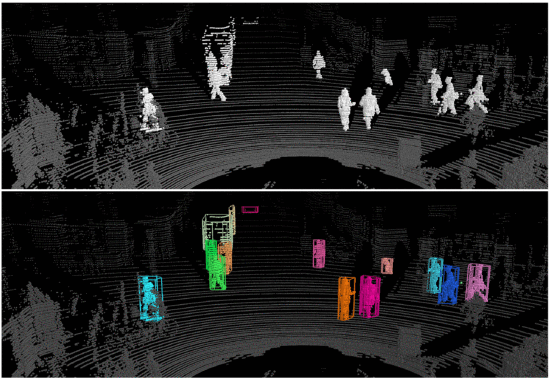
\includegraphics[width=0.7\linewidth]{images/pointcloudseg.png}
\caption{The class-agnostic instance-level segmentation over all foreground points performed by the proposed method }
\end{figure}

They carefully mix graph-theoretic algorithms with data-driven learning.
While data-driven learning is widely used due to its performance, it is
difficult to guarantee good results when processing out-of-sample data
from an open world. The proposed method searches over an exponentially
large space of possible segmentations and returns the one most similar
to the data-driven point-based model of ``objectness". First, the search
is restricted into a subset of segmentations that are consistent with a
hierarchical grouping of a point cloud sweep. Such hierarchical groups
can be readily produced with agglomerative clustering or hierarchical
graph-based algorithms. Since that a segmentation algorithm can produce
an exponentially-large set of segmentations, the authors introduce
efficient algorithms that search over a space of tree-consistent
segmentations and return the one that maximizes a global segmentation
score.

\subsection{Proposed approach}\label{header-n869}

For 3D object point segmentation, the input is a 3D point cloud, which
contains an \emph{unknown} number of objects. The goal is to produce a
point segmentation, in which every segment contains points from one and
only one object.

\subsubsection{Definitions}\label{header-n871}

A \emph{global segmentation} $P_X$ is a partition of a set of points
$X$ into subsets of points $C_i$ (called local segment), i.e
$P_X = \{C_i\}_{i = 1}^{M}$, where $M$ denotes the number of
segments and $C_i \subset X$. Importantly, every point exists in one
and only one segment.

The concept of \emph{tree-consistent segmentation} is defined as
follows. The set of all possible global segmentations on $X$ is
defined as $S_X$. Without constraints, the size of $S_X$ is
exponential but in practice the authors reduce the number of candidates
by enforcing geometric constraints. All points are grouped
hierarchically into a tree structure $T_X$. Now, the tree-consistent
segmentation is $S_{X,T}$ and contains all possible segmentation
defined by the tree $T$. The following figure illustrates the
relationship between $S_X$ and $S_{X,T}$.

\begin{figure}[h!]
\centering
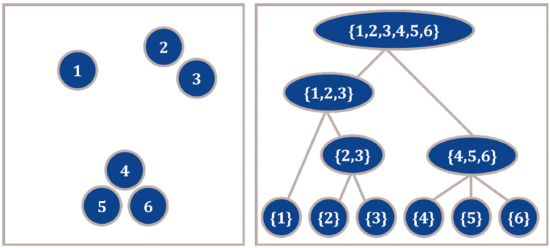
\includegraphics[width=0.7\linewidth]{images/treesegment.png}
\caption{Tree-consistent segmentation}
\end{figure}

Any tree-consistent segmentation from corresponds to a vertex cut set of
the tree $T$, i.e. a set of tree nodes, which satisfy the following
constraints:

\begin{itemize}
\item
  for each node in the vertex cut, its ancestor and itself cannot both
  be in the cut and
\item
  each leaf node must have itself or its ancestor in the cut. 
\end{itemize}

The \emph{segment score} is defined as a function $f(C, \theta)$,
where $C$ is the segment and $\theta$ are the function parameters.
$f$ predicts a given segment's ``objectness" and can be implemented by
a PointNet++, where $\theta$ are the network's weights.

The \emph{segmentation score} is calculated as the aggregation of the
score of all segments in a global segmentation $P_X$. Formally, given
a global segmentation $P_X = \{Ci\}^{M}_{i=1}$, its score is
$F(P_X; \theta) : PX→ [0, 1]$ by aggregating over local objectness of
all its segments.

\subsubsection{Worst-case segmentation}\label{header-n884}

The \emph{worst-case segmentation} score of a global segmentation is the
worst objectness among its local segments:

$ F_{\min }(P_X; \theta) = \min _i{f(C_i; \theta)}, i\in {1 \ldots M}.$

Now, the optimal worst-case segmentation is

$ P_{X,\min }^* = \mathop{\operatorname{argmax}}\limits_{P_X\in S_{X,T}} {F_{\min } (P_X; \theta)} $.

It turns out the problem of finding optimal worst-case segmentation has
optimal substructure, allowing us to find the global optimum efficiently
with dynamic programming (see the following figure).

\begin{figure}[h!]
\centering
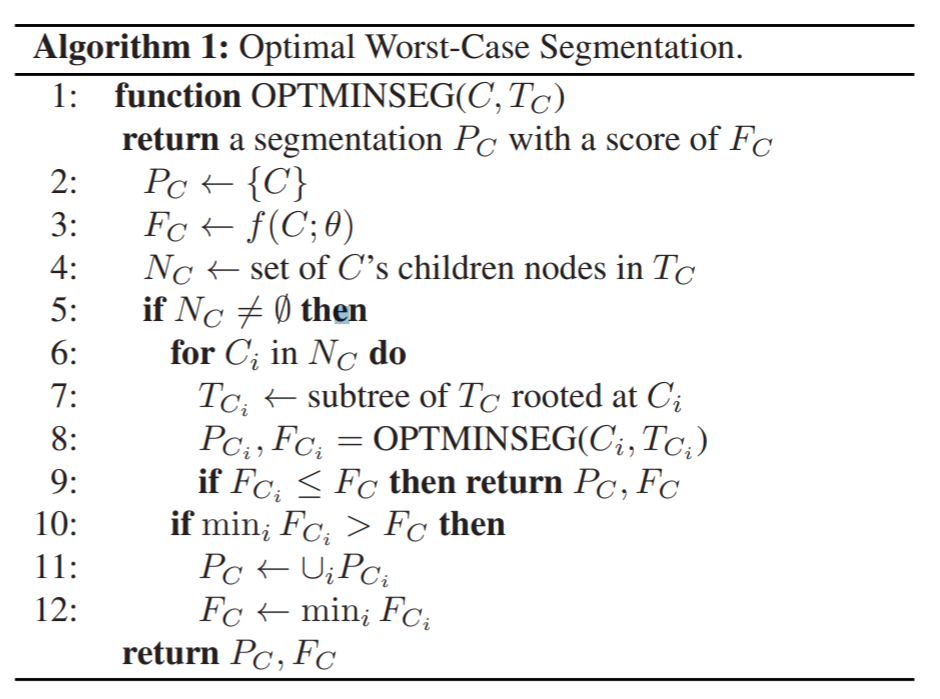
\includegraphics[width=0.8\linewidth]{images/worstcaseseg.png}
\caption{Optimal worst case segmentation}
\end{figure}

The algorithm starts from the root node $X$ and chooses between a
coarse segmentation and a fine one. The fine segmentation will be the
union of all $X$`s children's optimal worst-case segmentation, which
can be computed recursively. The algorithm would first traverse down to
the leaf nodes, representing the finest segmentation. Then it will make
its way up, during which it finalizes optimal segmentation for each
intermediate node by making local coarse vs. fine decisions. Eventually,
it returns to the root node and produces an optimal worst-case global
segmentation. This algorithm might not visit all nodes. Instead, it
skips a sub-trees whenever one sub-tree exhibits a lower score. The
algorithm's complexity is linear in $N$ despite the fact that the
search space is exponential in $N$.

\subsubsection{Average-case segmentation}\label{header-n892}

Average-case segmentation score of a global segmentation is the average
objectness among its local segments:
\newline
$ F_{\operatorname{avg}{}}(P_X; \theta) = \frac{1}{M} \sum _{i=1}^M f(C_i; \theta).$
\newline
$P_{X,\operatorname{avg}{}}^*$ can be defined as \emph{optimal
average-case segmentation} if
\newline
$ P_{X,\operatorname{avg}{}}^* = \mathop{\operatorname{argmax}}\limits_{P_X\in S_{X,T}} {F_{\operatorname{avg}{}} (P_X; \theta)}. $
\newline
It is important to specify that the problem of finding the optimal
average-case segmentation does not have optimal substructure, unlike
worst-case segmentation.

\subsubsection{Learning the Objectness Function}\label{header-n898}

Until now, the segmentation algorithms have been discussed under the
assumption that the objectness function $f(C; \theta)$ is defined (it
predicts an objectness score for a given point cloud). First of all, the
ground-truth function must be defined. Suppose to have the ground truth
segmentation $P^{gt} = \{C_1^{gt},...,C_L^{gt}\}$. To define the
target objectness of a segment, we have to consider that 3D sensors
(e.g. LiDAR) tend to produce denser points near the sensor. In
consequence, the objectness will be heavily influenced by the
partitioning of points closer to the sensor. A segment objectness
function of a segment is the largest point between itself and any ground
truth segment:
\newline
$ Objectness(C, P^{gt}) = \max _{l=1,\ldots,L} \frac{\sum _{x \in C \cap C^{gt}_l} x^T x }{\sum _{x \in C \cup C^{gt}_l} x^T x }, $
\newline
where $x^T x$ represents the squared distance of a point $x$ to
sensor origin. The authors train a PointNet++ model for learning the
objectness function. Each segment is re-sampled to 1024 points.

\subsubsection{Building tree hierarchies}\label{header-n902}

This section explains how to build a tree structure given a set of
points $X$. One natural approach is agglomerative clustering, merging
points in classes according to their spatial features. This approach
tends to create tree hierarchies with very fine granularity, e.g. one
node may differ from another with only one point of difference. In this
work, the authors propose a method which builds a coarser tree whose
leaf nodes are segments (rather than individual points) and adjacent
nodes should differ from each other much more. To build such a tree,
Euclidean Clustering algorithm is used recursively in a top-down fashion
with a list of decreasing $\epsilon$. In the beginning, the algorithm
is run with the largest $\epsilon$ value, defining the most coarse
connected components. Then, the procedure is repeated a smaller
$\epsilon$ within each connected component. This produces a
multiple-tree top-down hierarchy.

\subsection{Experiments}\label{header-n904}

For evaluation, the authors repurpose the KITTI object detection
benchmark for point cloud segmentation, following the setup in {[}30{]}.
The ground truth segmentation is composed of a series of point segments
marked with a bounding box. All the background points (those outside the
bounding box) are removed. To evaluate the performance are considered
two metrics: the \emph{under-segmentation error} $U$ and the
\emph{over-segmentation error} $O$, defined as follows:
\newline
$ U = \frac{1}{L} \sum _{l=1}^L \mathbf {1} \left(\frac{|C_{i^*} \cap C_l^{gt}|}{|C_{i^*}|} < \tau _U\right) \\ O = \frac{1}{L} \sum _{l=1}^L \mathbf {1} \left(\frac{|C_{i^*} \cap C_l^{gt}|}{|C_l^{gt}|} < \tau _O\right)$
\newline
with
\newline
$ i^* = \operatorname{argmax}_{i=1}^M{|C_i \cap C^{gt}_l|}$
\newline
and $\tau _U, \tau _O$ as constant thresholds, set to
$\frac{2}{3}, 1$.
\newline
The Euclidean clustering algorithm is applied with an
$\epsilon \in \{2 m, 1 m, 0.5 m, 0.25 m\}$. The authors include it as
a baseline to find better solutions. As baselines, other
state-of-the-art 3D detectors are included: AVOD, PointPillars,
PointRCNN, and SECOND. Since these detectors output class-specific
bounding box detection, the authors simply ignore the class label to
produce class-agnostic segmentations. In addition, the authors include
for evaluation modified versions of the proposed baselines, in order to
improve their performance. A much better approach, called
\emph{\{Detector\}++} (e.g. AVOD++ etc.), check if the leftover segments
can be included in an existing detection segment. Another approach,
SECOND++, consists of re-train and re-evaluate the best baseline, i.e.
SECOND, with background removal. These baselines are marked with ``+ BG
Removal". In addition, the authors discover that, by extending the
SECOND's detection range from 50 m to 80 m, the SECOND's performance is
significantly improved. The affected baselines are marked with ``+ Ext.
Range". Finally, they re-train and re-evaluate SECOND on all 8 classes.
The new baselines are labeled as ``SECOND++(8)", while the off-the-shelf
SECOND baselines are labeled as ``SECOND++(4)". The following figure
resumes the results obtained.

\begin{figure}[h!]
\centering
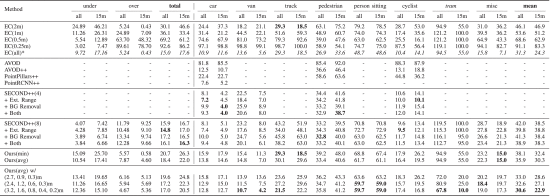
\includegraphics[width=1\linewidth]{images/segmentationerrors.png}
\caption{Segmentation errors on the proposed method (*Ours*) and the baselines}
\end{figure}

The table shows that the average-case segmentation, \emph{Ours(avg)},
consistently outperforms the optimal worst-case segmentation
\emph{Ours(min)}. \emph{Ours(min)} produces a much lower
over-segmentation error but a much higher under-segmentation error,
suggesting it makes more mistakes of grouping different objects into one
segment and fewer mistakes of splitting points from one single object
into multiple segments. The authors label Euclidean Clustering as
``EC()," where $\epsilon$ represents the distance threshold (meter) and
constructs a pool of segments that contains every node (segment) in the
hierarchy and call this ``EC(all)*". This serves as an unreachable
upper-bound. The gap between our proposed method and the upper bound is
relatively small (3--4\%), suggesting plenty of room left for
improvement in creating better hierarchies. The confront between a
\emph{Detector} algorithm and its variation \emph{Detector++}, shows
that the improved version obtains better performance (see the AVOD's
case). SECOND++ performs the best among all Detector++ baselines.
SECOND++ performs better on common classes such as cars while the
proposed method perform better on rare ones such as misc. Another
evaluation metric is measure how objectness generalizes over different
classes. The authors apply the learned objectness onto truth segments
from the validation set. The graph below shows the results.

\begin{figure}[h!]
\centering
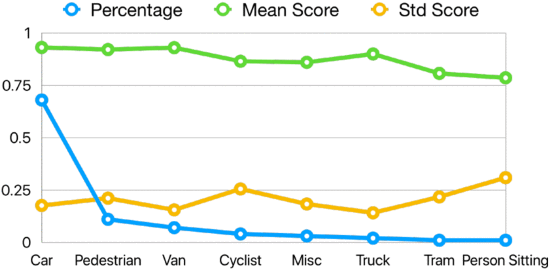
\includegraphics[width=0.8\linewidth]{images/objectnessgen.png}
\caption{Learned objectness generalization}
\end{figure}

As the number of training data decreases dramatically, the average score
tends to drops slightly and the variance tends to rise slightly. In
conclusion, the authors prove that their algorithm is guaranteed to
achieve optimality to a specific definition. On KITTI, the proposed
approach significantly outperforms past bottom-up approaches and
top-down object-based algorithms for segmenting point clouds.
\newpage

\section{Multi-View Incremental Segmentation of 3-D Point Clouds for
Mobile Robots}\label{header-n915}

\emph{IEEE ROBOTICS AND AUTOMATION LETTERS, VOL. 4, NO. 2, APRIL 2019}
{[}31{]}

\subsection{Introduction}\label{header-n917}

Mobile robots are frequently used to autonomously explore and survey
unknown areas. To understand an environment, a robot can use a 3D sensor
to acquire data in point cloud form. A point cloud is an array of 3D
points containing geometric and optionally color information. This type
of data can be used for many different purposes, the one treated in this
work is the semantic segmentation of the environment. The initial
approaches used to perform point cloud segmentation are
clustering-based. Clustering methods usually rely on generating seed
points, and subsequently, create a point cloud cluster around it. The
point can be grouped considering different features, like distance
and/or color. On the other hand, classification of point cloud data can
be carried out: in this way each point has an individual label. Some
methods project the 3D point cloud into a 2D form and perform
segmentation on the resulting image. Other methods use 3D convolutions
and others use both geometrical and scene features. Further advancements
to this line of work use, recurrent networks, or coarse-to-fine
hierarchies to incorporate neighborhood information and local
dependencies to the prediction stage. However, these methods operate on
point clouds one at a time and do not incorporate information from new
scans or they are performed offline after complete point cloud data is
obtained. In particular, semantic segmentation is usually performed on
individual scans or performed offline after complete scan data is
collected. To overcome these shortcomings, this study proposes a
multi-view incremental segmentation method that can perform online
instance segmentation of 3D point clouds. A neural network assigns a
label to each point and the segmentation results are progressively
updated. The key idea is to consider a select few of the previous scans,
to improve the segmentation of the current scan.

\subsection{Proposed method}\label{header-n919}

The test and training data are obtained from the Stanford 3D Indoor
Spaces (S3DIS) dataset. In contains 6 building areas with point clouds
segments individually annotated. It also contains 13 classes of objects,
like walls, chairs, doors, and other types of furniture. A virtual robot
with laser scanners is placed in the environment and acquires laser
scans by ray-tracing. The robot is also equipped with cameras so that
color information can be mapped onto the point cloud. The robot acquires
a scan every $2m$ and ray-tracing is carried out. The figure below
shows the original point cloud of a room as well as the resulting point
cloud obtained by ray-tracing along a trajectory.

\begin{figure}[h!]
\centering
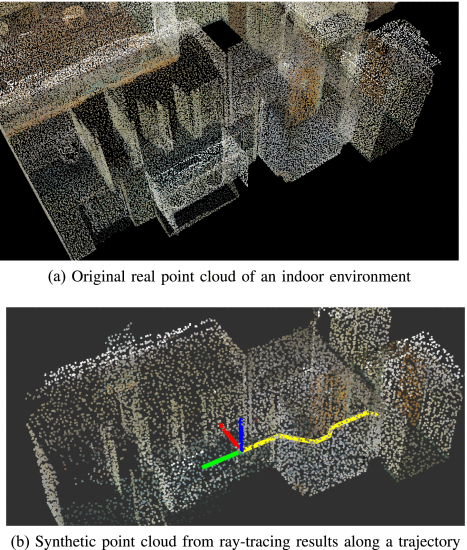
\includegraphics[width=0.7\linewidth]{images/pointclouds.png}
\caption{Visualization of dynamic scanning by ray-tracing for a virtual mobile robot}
\end{figure}

The proposed incremental segmentation method involves a neural network
architecture, named Multi-view Context Pooling Network (MCPNet), that
jointly predicts an instance label and a class label for each scanned
point. The class label describes the semantic class of a point (i.e.
wall, door, table, etc.) whereas the instance label is a unique ID such
that only points from the same object instance have the same ID. In an
online segmentation procedure, it is important to keep track of newly
scanned points and their relationship to previously scanned points.
Thus, a voxel grid with a grid size of $0.1m$ is used as a lookup
table to store the point coordinates and their corresponding
segmentation results: the point cloud is limited to one point per voxel.
First, each input scan considers as a valid point only those in an area
of radius $2m$ around the robot (points discarded will be considered
in future scans). Next, the point coordinates are normalized so that the
x-y coordinates are centered around the robot and the z-coordinate is
zero at the floor level. The points are then divided into batches of
$N\times 6$ matrices, where $N$ is the batch size and the columns
are X-Y-Z-R-G-B values. These matrices are passed to the network.
MCPNet's architecture is reported in the following figure.

\begin{figure}[h!]
\centering
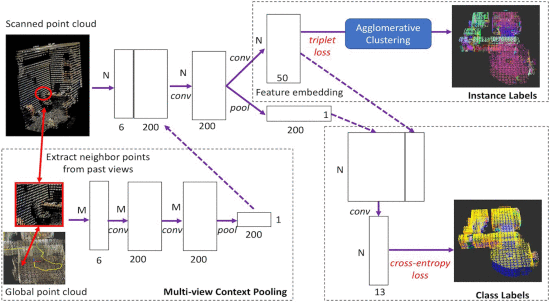
\includegraphics[width=0.91\linewidth]{images/MCPNetarc.png}
\caption{MCPNet architecture for incremental instance segmentation of 3D point clouds}
\end{figure}

The input matrix is first passed through a 1D convolution layer to form
an intermediate $N\times 200$ feature matrix. The network then splits
into two branches: the lower branch for classification and the upper
branch for clustering. The \emph{lower branch} uses a max-pooling
function to compute a global feature vector representing the input
points. This is then concatenated with the feature embedding from the
upper branch and passed through another 1D convolution layer to compute
class probabilities for each point, represented as a $N\times 13$
matrix since there are 13 classes. The \emph{upper branch} aims to
project the point features to an embedding space that is suitable for
clustering. This is enforced by computing a triplet loss between sets of
three points, $p_1$ , $p_2$ which originate from the same object and
$p_3$ which originates from a different object and minimizing the
resulting loss function (the projection is a function
$f : \R^{3} \rightarrow \R^{50}$). At training time, minimizing the
triplet loss encourages the distance between points that should belong
to the same object to be greater than that of points that should belong
to different objects in the embedding space, i.e.
$\parallel f(p_1) - f(p_2)\parallel^{2} + \alpha < \parallel f(p_1) - f(p_3)\parallel^{2}$,
where $\alpha$ is the margin parameter. At inference time, fo each
point $p_i$ a set of neighbor points are retrieved (points that is at
most one cell away from $p_i$). Then, each point $p_i$ is only
connected to a neighboring point $p_j$ if the cosine similarity
\newline
$\frac{f(p_i) \cdot f(p_j)}{\parallel f(p_i)\parallel \parallel f(p_j)\parallel}$
\newline
is greater than $\beta$ (a preset threshold). The following rules are
then applied:

\begin{itemize}
\item
  if no connections exist, the point is initialized as the seed for a
  new cluster with a new instance ID; 
\item
  if connections exist to a single existing cluster, the point is added
  to that cluster and takes the corresponding instance ID;
\item
  if connections exist to multiple existing clusters, all connected
  clusters are merged and their instance IDs are updated accordingly.
\end{itemize}

The \emph{Multi-view Context Pooling} (MCP) module incorporates
contextual information from previous views to improve the classification
accuracy. The input to the MCP module is an $N\times M\times 6$ tensor
that stores context points for each of the $N$ points in the current
input (only $M$ points from previous scans are considered). A context
point for point $p_i$ is defined as any point from previous views that
is at most three cells away from $p_i$ in the global voxel grid.

\subsection{Experiments results}\label{header-n935}

The instance segmentation results were first evaluated in terms of the
classification accuracy on the S3DIS dataset, where one area of the
dataset is held out as test data whereas the remaining areas are used as
training data. The proposed method are compared with other conventional
approaches: PointNet {[}14{]}, PointNet++ {[}32{]}, VoxNet {[}33{]} and
SGPN. The evaluation metrics are:

\begin{itemize}
\item
  \textbf{Intersection-Over-Union (IOU):} it is defined as the number of
  true positive points divided by the total true positive, false
  positive, and false negative points.
\item
  \textbf{Point-wise Accuracy:} it is the number of true positive points
  divided by the total number of points.
\item
  \textbf{Object-wise Accuracy:} defined as the number of true positive
  object instances divided by the total number of object instances.
\end{itemize}

The table below shows the results obtained.

\begin{figure}[h!]
\centering
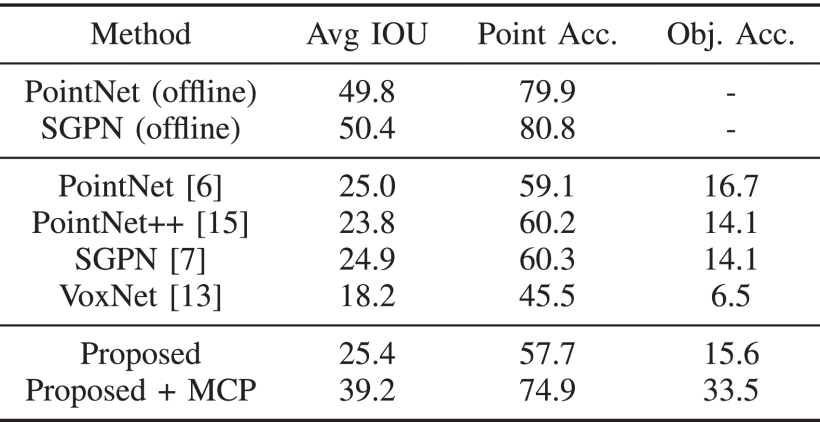
\includegraphics[width=0.7\linewidth]{images/segresultsaccu.png}
\caption{Classification accuracy on S3DIS dataset}
\end{figure}

Experimental results show that the proposed method with MCP outperforms
the other methods in terms of both IOU and accuracy. The authors
performed also an analysis of the effect of the number of the context
points used in the proposed MCP module on the classification accuracy.
The following graph shows that the average accuracy increases with
number of context points but also incurs a higher computational cost.
\newpage
\begin{figure}[h!]
\centering
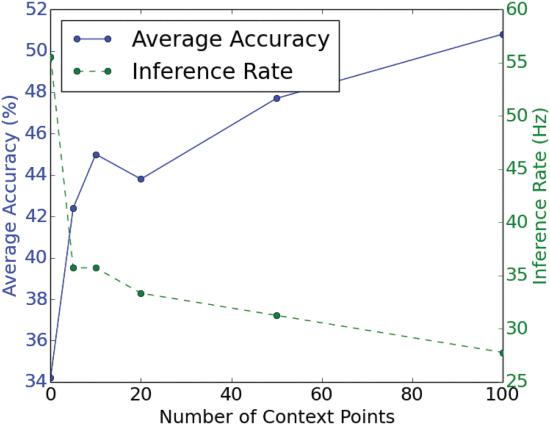
\includegraphics[width=0.7\linewidth]{images/MCPpoints.png}
\caption{Classification accuracy and inference rate as a function of the number of context points}
\end{figure}

On the other hand, the clustering performance was measured using three
different metrics: normalized mutual information (NMI), adjusted mutual
information (AMI), and adjusted rand index (ARI), as defined in
{[}35{]}. In particular, PointNet, PointNet++, and VoxNet used a
clustering technique in which connected components are formed between
points with the same class label, while the remaining methods used the
agglomerative clustering technique described in this work, with
$\beta = 0.98$ for SGPN and $\beta = 0.9$ for MCPNet. The table
below shows the results obtained.

\begin{figure}[h!]
\centering
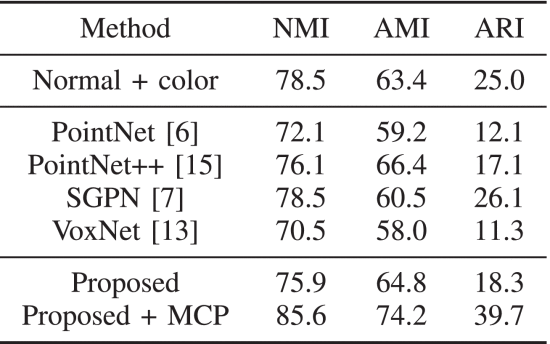
\includegraphics[width=0.65\linewidth]{images/clusper.png}
\caption{Clustering performance on S3DIS dataset}
\end{figure}

Results show that even the simple normal + color-based region-growing
scheme can achieve a good clustering, but the proposed method with MCP
achieved the best clustering result overall. The following figure shows
the global instance segmentation results at intermediate points along
the incremental scanning process: input point cloud with virtual robot
trajectory (top row), clustering results (middle row) and classification
results (bottom row).

\begin{figure}[h!]
\centering
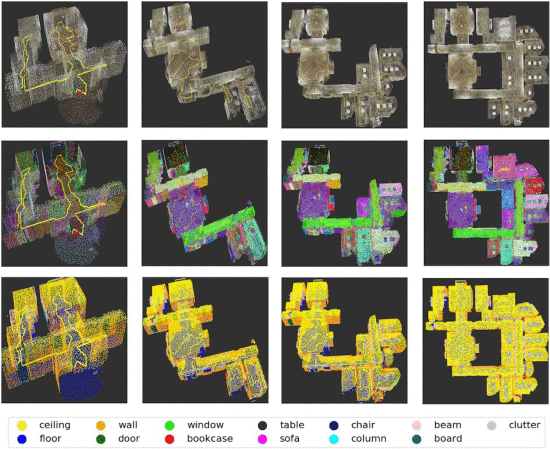
\includegraphics[width=0.7\linewidth]{images/incremseg.png}
\caption{Incremental segmentation results on S3DIS test dataset}
\end{figure}

Experimental results show that the proposed approach led to 15\%
improvement in accuracy and 7\% improvement in NMI compared to the next
best online method.
\newpage

\section{Real Time Trajectory Prediction Using Deep Conditional
Generative Models}\label{header-n953}

\emph{IEEE ROBOTICS AND AUTOMATION LETTERS, VOL. 5, NO. 2, APRIL 2020}
{[}36{]}

\subsection{Introduction}\label{header-n955}

Dynamic high-speed robotics tasks often require accurate methods to
forecast the future value of a physical quantity and these methods must
respect the application's real-time constraints. For example, to hit or
catch a flying ball, a robot needs to predict accurately and fast the
trajectory of the ball. Note that the time it takes to compute the
predictions, called \emph{latency}, is as important for the application
as the accuracy in the prediction. Physics-based models are often used
to trajectory forecasting because of their velocity in making a
prediction. Despite this, in some applications, the best known
physics-based model is not accurate enough or, even if the physics is
accurate, estimating all its relevant variables can be difficult. On the
other hand, a data-driven model could overcome these limitations and,
generally, their predictions are more accurate. However, the modern
data-driven approaches, like those based on recurrent neural networks,
suffer from cumulative errors. This work proposes a novel method for
trajectory prediction that mixes the power of deep learning and
conditional generative models to provide a data-driven approach for
accurate trajectory forecasting with the low latency required by
real-time applications. The system is tested using a table tennis
system, in which two robotic arms has to correctly hit a ball. The
figure below shows this system.

\begin{figure}[h!]
\centering
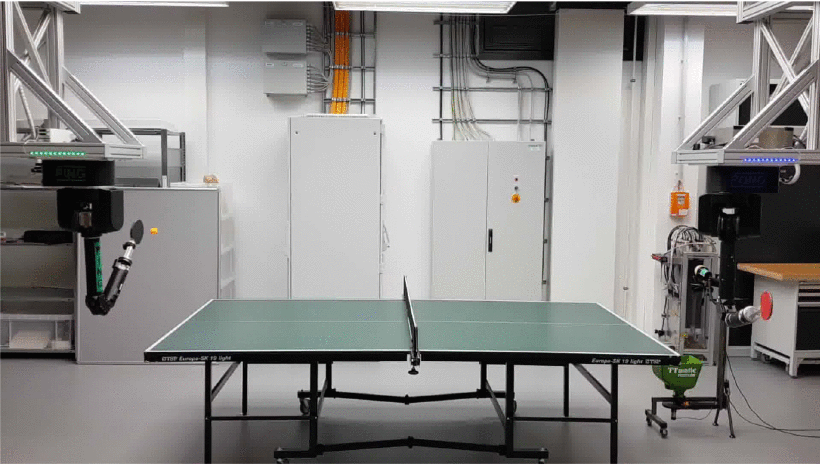
\includegraphics[width=0.7\linewidth]{images/tabletennis.png}
\caption{Table tennis robotic system}
\end{figure}

\subsection{Proposed method}\label{header-n958}

\subsubsection{Trajectory definition}\label{header-n959}

The term trajectory is commonly used to refer to a realization of a time
series or Markov decision process. A trajectory is defined as
$\tau=\{y_t^{n}\}^{T_n}_{t=1}$, where $T_n$ is a sequence of
multiple observations $y_t^{n}$ ($n$ represents the time and $t$
is the index of a trajectory in the data set). For the tennis example,
an observation $y^{n}_t$ is a three-dimensional vector representing
the ball position at time $t$ of the ball trajectory $n$. Each
trajectory $\tau_n∼ P(\tau)$ is assumed to be independently sampled
from the trajectory distribution $P(\tau)$. Formally, the goal of
trajectory forecasting is to compute the conditional distribution
$p(y_t,..., y_T | y_1,..., y_{t−1})$, representing the distribution of
the future values of a trajectory $\{y_t,..., y_T \}$ given the
previous observations $\{y_1,...., y_{t-1}\}$ ($y_t$ is a random
variable representing the observation indexed by time $t$ in any
trajectory). Some models use the factorization property of probability
theory
\newline
$ p(\boldsymbol{y}_{t:T} \, | \,\boldsymbol{y}_{1:t-1}) = \prod _{i=t}^{T}{p(\boldsymbol{y}_{i} \, | \,\boldsymbol{y}_{1:i-1})}, $
\newline
but they predict directly a single observation, while the others are
calculated by using the past predictions as input. This is a
\emph{recursive} approach: it uses its predictions as input to predict
farther into the future. These approaches can predict sequences of
arbitrary length, but they have the disadvantage that errors are
cumulative. However, for trajectory prediction in physical systems,
where we are measuring all the relevant variables, the authors would
expect long term prediction to be more accurate. In fact, this is not
true and even a data-driven model, implemented for example with LTSM, is
heavily penalized by the cumulative error, that renders long term
predictions less accurate.

\subsubsection{Deep conditional generative models}\label{header-n963}

The goal is to find a way to represent the conditional distribution
$p(y_{t:T} | y_{1:t−1})$ directly, in a way where the model
predictions are not fed back into the model. In addition, we want to use
a powerful model that can capture non-linear relationships between the
future and past observations. To do this, a complex non-linear
regression model, such as a neural network, can be used. The authors use
two auxiliary input variables $x^{t}$ and $\hat x^{t}$ that
represent a zero-padded input observation and an observation mask. In
particular, $x^{t} = 1$ represent the observations viewed so far,
while the non-observed parts of the trajectory are tagged with
$x^{t} = 0$. Similarly, the variable $\hat x^{t} \in \{0, 1\}$
indicates which values were observed and which values were not. Using
the auxiliary variables the model can make predictions with any number
of input observations $t \in \{0, 1,...,T\} $. The proposed approach
assumes a fixed maximum prediction horizon $T$ for all trajectories.

\subsubsection{Capturing Uncertainty and Variability}\label{header-n965}

Quantifying the uncertainty of the trajectory predicted by the model is
important for decision making. In robot table tennis, for example, the
robot could wait for more ball observations if there is high uncertainty
about the ball trajectory, but waiting too long will result in failure
to hit the ball. Uncertainty can be captured using a latent variable
$z_n$, that can be mapped to a trajectory using a complex non-linear
function. The authors want to emphasize that the limitation of a fixed
prediction horizon $T$ means that prediction beyond $T$ can't be
done, but the model can be trained with trajectories of any length
$T_n$. The proposed approach is based on variational auto-encoders.
The decoder network takes as input the previous observations
$y_{1:t−1}$ represented by $(x^{t} , \hat x^{t} )$ as well as the
latent variable $z$ that encodes one of the possible future
trajectories $\hat y$ (which contains the predicted future
observations $y_{t:T}$. The encoder network produces the variational
distribution $q\varphi(z | y1:t)$, which is a partial trajectory with
observations $y_{1:t}$ to the latent space $z$.

\begin{figure}[h!]
\centering
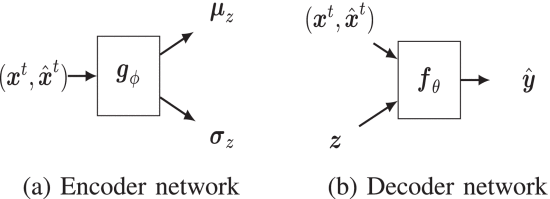
\includegraphics[width=0.8\linewidth]{images/encdec.png}
\caption{Encoder and decoder networks for the proposed approach}
\end{figure}

\subsubsection{Inference and training procedure}\label{header-n968}

At prediction time, the encoder computes the latent space distribution
using the given past observations. It produces a mean $\mu_z$ and a
standard deviation $\sigma_z$. Next, several values
$z^l \sim {\mathcal N}(z | \mu_z, \sigma_z)$ are sampled and they are
passed, with the past observations, to the decoder module to predict the
future trajectory. The training set consists of a set of trajectories
$\tau_n$ each of a possibly different length $T_n$. Sampled
mini-batches are used to train the model: for any trajectory, a cut
point $t : 0 <t $ is randomly selected and the lower bound for
$p(y_{t:T} | y_{1:t−1})$ is computed for the particular $t$. In this
way, the model will learn to make predictions for any number of given
observations, including an empty set. Finally, to make our model more
robust, the authors randomly generate missing observations and outliers
for the previous observations $y_{1:t−1}$ in each of the trajectories
included in the training mini-batch. To generate outliers, an
observation is simply replaced with a random value within the input
domain.

\subsection{Experiments}\label{header-n970}

The authors evaluate the proposed method (which predicts the trajectory
of a table tennis ball) both in a real and simulated system. The
proposed method is called "TVAE" (Trajectory Variational Auto-Encoder).
The metric measured is the prediction error and latency. The baseline
methods, used to compare and evaluate the performance of the proposed
method, are an LTSM and the physics-based approach. The ball's physics
is described in {[}37{]}, while the initial velocity and position are
calculated as described in {[}38{]}. The latter method consists of
fitting a polynomial to the first $n$ observations and evaluating the
polynomial of degree $k$ and its derivative in $t = 0$. These
parameters are set to $n = 30$ and $k = 2$, that provided the
highest predictive performance on the training data set.

\subsubsection{Prediction accuracy in simulation}\label{header-n972}

The results should be optimal for the physics-based model on simulation,
where the only source of error is the initial position and velocity
estimation from noisy ball observations. The authors generated 2000 ball
trajectories for training and another 200 for the test. The training
results obtained in a simulated environment are plotted in the following
figure. In simulation, the error distribution of the proposed method and
the physics-based model is almost identical. The results of the LSTM are
slightly better than the proposed model for the first 10 observations,
but the error for long term prediction grows uncontrollably.

\begin{figure}[h!]
\centering
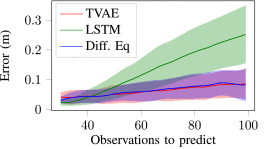
\includegraphics[width=0.37\linewidth]{images/accuracyballres.png}
\caption{Distribution of the error in the test set for simulated data as a function of the number of observations}
\end{figure}

\subsubsection{Prediction accuracy in the real
system}\label{header-n975}

There are several issues that make ball prediction harder on the real
system: there are missing observations, the error is not the same in all
the space due to the effects of lens distortion, and the ball spin can
not be observed directly. The training set has 614 samples, while the
test set is composed of 35 trajectories. All samples are collected in a
real environment: the ball is thrown using the hand, using a mechanical
launcher, and hitting them with a table tennis racket. Since the
trajectories have typically a duration between 0.8 and 1.2 seconds, the
time horizon is set to $T = 1.2$ seconds. The figure below shows the
training results obtained using real-time data. The proposed method
outperforms the long term prediction accuracy of the other models. The
LSTM, as expected, is very precise at the beginning but starts to
accumulate errors and becomes quickly less accurate. The physics-based
model is in the middle: more accurate than the LTSM approach but less
accurate than TVAE.

\begin{figure}[h!]
\centering
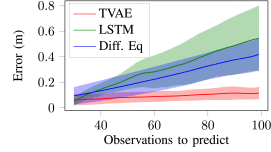
\includegraphics[width=0.37\linewidth]{images/accuracyballresreal.png}
\caption{Distribution of the error in the test set for real data as a function of the number of observations}
\end{figure}

\subsubsection{A real robot table tennis system}\label{header-n978}

The authors implemented the proposed method in a real robot table tennis
system, to test the performance in a real game. To do this, they
modified the ProMP approach {[}39{]} to use the proposed ball model.
ProMP works as follows:

\begin{itemize}
\item
  first, the initial time and duration of the movement primitive are
  computed by maximizing the likelihood of hitting the ball;
\item
  second, the movement primitive is adapted to hit the ball using a
  probability distribution by conditioning the racket distribution to
  intersect the ball distribution;
\item
  third, to avoid dangerous movements, the robot does not hit if the
  likelihood is lower than a certain threshold.
\end{itemize}

To compute the ball distribution, the authors took 30 trajectory samples
from the proposed model and computed empirically its mean and
covariance. The adapted method obtained a hitting rate of 98.9\%
compared to 96.7\% obtained using a ProMP. This experiment also shows
that the presented approach can be used in a system with hard real-time
constraints. The proposed system can infer the future ball trajectory
from past observations with a latency between 8 ms and 10 ms.
\newpage


\begin{thebibliography}{99}
\bibitem{} Niko Sünderhauf, Oliver Brock, Walter Scheirer, Raia Hadsell,
Dieter Fox, Jürgen Leitner, Ben Upcroft, Pieter Abbeel, Wolfram Burgard,
Michael Milford, Peter Corke, ``The Limits and Potentials of Deep
Learning for Robotics", eprint arXiv:1804.06557, April 2018

\bibitem{} A. Giusti \emph{et al}., ``A Machine Learning Approach to Visual
Perception of Forest Trails for Mobile Robots," in \emph{IEEE Robotics
	and Automation Letters}, vol. 1, no. 2, pp. 661-667, July 2016, doi:
10.1109/LRA.2015.2509024.

\bibitem{} P. Santana, L. Correia, R. Mendonça, N. Alves, and J. Barata,
``Tracking natural trails with swarm-based visual saliency," J. Field
Rob., vol. 30, no. 1, pp. 64--86, 2013.

\bibitem{} M. Chancán, L. Hernandez-Nunez, A. Narendra, A. B. Barron and M.
Milford, ``A Hybrid Compact Neural Architecture for Visual Place
Recognition," in \emph{IEEE Robotics and Automation Letters}, vol. 5,
no. 2, pp. 993-1000, April 2020, doi: 10.1109/LRA.2020.2967324.

\bibitem{} A. Magassouba, K. Sugiura, A. Trinh Quoc, and H. Kawai,
``Understanding natural language instructions for fetching daily objects
using GAN-based multimodal target-source classification," IEEE Robot.
Autom. Lett., vol. 4, no. 4, pp. 3884--3891, Oct. 2019.

\bibitem{} H. Fukui, T. Hirakawa, T. Yamashita, and H. Fujiyoshi,
``Attention branch network: Learning of attention mechanism for visual
explanation," in Proc. CVPR, 2019, pp. 10 705--10 714.

\bibitem{} J. Hatori et al., ``Interactively picking real-world objects with
unconstrained spoken language instructions," in Proc. IEEE ICRA, 2018,
pp. 3774--3781.

\bibitem{} A. Palffy, J. Dong, J. F. P. Kooij and D. M. Gavrila, ``CNN Based
Road User Detection Using the 3D Radar Cube," in \emph{IEEE Robotics and
	Automation Letters}, vol. 5, no. 2, pp. 1263-1270, April 2020, doi:
10.1109/LRA.2020.2967272.

\bibitem{} W. Liu et al., ``SSD: Single shot multibox detector," Lecture
Notes in Computer Science (including subseries Lecture Notes in
Artificial Intelligence and Lecture Notes in Bioinformatics), vol. 9905
LNCS, pp. 21--37, 2016.

\bibitem{} R. Prophet et al., ``Pedestrian classification with a 79 GHz
automotive radar sensor,'' in Proc. 19th Int. Radar Symp., 2018, pp.
1--6.

\bibitem{} O. Schumann, M. Hahn, J. Dickmann, and C. Wöhler, ``Comparison
of random forest and long short-term memory network performances in
classification tasks using radar," in Proc. Sensor Data Fusion: Trends,
Solutions, Appl., 2017, pp. 1--6.

\bibitem{} A. Kurobe, Y. Sekikawa, K. Ishikawa and H. Saito, ``CorsNet: 3D
Point Cloud Registration by Deep Neural Network," in \emph{IEEE Robotics
	and Automation Letters}, vol. 5, no. 3, pp. 3960-3966, July 2020, doi:
10.1109/LRA.2020.2970946.

\bibitem{} P. J. Besl and N. D. McKay, ``Method for registration of 3-d
shapes," in Proc. Sensor Fusion IV: Control Paradigms Data Struct.,
1992, vol. 1611, 1992, pp. 586--607.

\bibitem{} C. R. Qi, H. Su, K. Mo, and L. J. Guibas, ``Pointnet: Deep
learning on point sets for 3d classification and segmentation," in Proc.
IEEE Conf. Comput. Vis. Pattern Recognit., 2017, pp. 652--660.

\bibitem{} Y. Aoki, H. Goforth, R. A. Srivatsan, and S. Lucey,
``Pointnetlk: Robust \& efficient point cloud registration using
pointnet," IEEE Conf. Comput. Vis. Pattern Recog. (CVPR), Jun. 2019.

\bibitem{} Z. Wu et al., ``3D shapenets: A deep representation for
volumetric shapes," in Proc. IEEE Conf. Comput. Vis. Pattern Recognit.,
2015, pp. 1912--1920.

\bibitem{} M. Mancini, S. R. Bulò, E. Ricci and B. Caputo, ``Learning Deep
NBNN Representations for Robust Place Categorization," in \emph{IEEE
	Robotics and Automation Letters}, vol. 2, no. 3, pp. 1794-1801, July
2017, doi: 10.1109/LRA.2017.2705282.

\bibitem{} I. Kuzborskij, F. Maria Carlucci, and B. Caputo, ``When naive
bayes nearest neighbors meet convolutional neural networks," in Proc.
IEEE Conf. Comput. Vis. Pattern Recognit., 2016, pp. 2100--2109.

\bibitem{} A. Krizhevsky, I. Sutskever, and G. E. Hinton, ``Imagenet
classification with deep convolutional neural networks," in Proc. 25th
Int. Conf. Neural Inf. Process. Syst., 2012, pp. 1097--1105.

\bibitem{} Y. Jia et al., ``Caffe: Convolutional architecture for fast
feature embedding," in Proc. 22nd ACM Int. Conf. Multimedia, 2014, pp.
675--678.

\bibitem{} K. Simonyan and A. Zisserman, ``Very deep convolutional networks
for large-scale image recognition," 2014, arXiv preprint arXiv:
1409.1556.

\bibitem{} C. Szegedy et al., ``Going deeper with convolutions," in Proc.
IEEE Conf. Comput. Vis. Pattern Recognit., 2015, pp. 1--9.

\bibitem{} B. Zhou, A. Lapedriza, J. Xiao, A. Torralba, and A. Oliva,
``Learning deep features for scene recognition using places database," in
Proc. 27th Int. Conf. Neural Inf. Process. Syst., 2014, pp. 487--495.

\bibitem{} B. Zhou, A. Khosla, A. Lapedriza, A. Torralba, and A. Oliva,
``Places: An image database for deep scene understanding," 2016, arXiv
preprint arXiv: 1610.02055.

\bibitem{}A. Pronobis, B. Caputo, P. Jensfelt, and H. I. Christensen, ``A
discriminative approach to robust visual place recognition," in Proc.
IEEE/RSJ Int. Conf. Intell. Robots Syst., 2006, pp. 3829--3836.

\bibitem{} J. Wu and J. M. Rehg, ``Centrist: A visual descriptor for scene
categorization," IEEE Trans. Pattern Anal. Mach. Intell., vol. 33, no.
8, pp. 1489--1501, Aug. 2011.

\bibitem{} E. Fazl-Ersi and J. K. Tsotsos, ``Histogram of oriented uniform
patterns for robust place recognition and categorization," Int. J.
Robot. Res., vol. 31, no. 4, pp. 468--483, 2012.

\bibitem{} P. Hu, D. Held and D. Ramanan, ``Learning to Optimally Segment
Point Clouds," in \emph{IEEE Robotics and Automation Letters}, vol. 5,
no. 2, pp. 875-882, April 2020, doi: 10.1109/LRA.2020.2965389.

\bibitem{} A. Magassouba, K. Sugiura and H. Kawai, ``A Multimodal
Target-Source Classifier With Attention Branches to Understand Ambiguous
Instructions for Fetching Daily Objects," in IEEE Robotics and
Automation Letters, vol. 5, no. 2, pp. 532-539, April 2020, doi:
10.1109/LRA.2019.2963649.

\bibitem{} D. Held, D. Guillory, B. Rebsamen, S. Thrun, and S. Savarese,
``A probabilistic framework for real-time 3D segmentation using spatial,
temporal, and semantic cues," Robotics: Science and Systems, 2016.

\bibitem{} J. Chen, Y. K. Cho and Z. Kira, ``Multi-View Incremental
Segmentation of 3-D Point Clouds for Mobile Robots," in \emph{IEEE
	Robotics and Automation Letters}, vol. 4, no. 2, pp. 1240-1246, April
2019, doi: 10.1109/LRA.2019.2894915.

\bibitem{} C. R. Qi, L. Yi, H. Su, and L. J. Guibas, ``Pointnet++: Deep
hierarchical feature learning on point sets in a metric space,"
arXiv:1706.02413, 2017.

\bibitem{} D. Maturana and S. Scherer, ``VoxNet: A 3D convolutional neural
network for real-time object recognition," in Proc. IEEE/RSJ Int. Conf.
Intell. Robot Syst., 2015, pp. 922--928.

\bibitem{} W. Wang, R. Yu, Q. Huang, and U. Neumann, ``SGPN: Similarity
group proposal network for 3D point cloud instance segmentation," in
Proc. IEEE Conf. Comput. Vis. Pattern Recognit., Jun. 2018, pp.
2569--2578.

\bibitem{} N. X. Vinh, J. Epps, and J. Bailey, ``Information theoretic
measures for clusterings comparison: Variants, properties, normalization
and correction for chance,'' J. Mach. Learn. Res., vol. 11, pp.
2837--2854, Dec. 2010. {[}Online{]}. Available:
http://dl.acm.org/citation.cfm?id=1756006.1953024.

\bibitem{} S. Gomez-Gonzalez, S. Prokudin, B. Schölkopf and J. Peters,
``Real Time Trajectory Prediction Using Deep Conditional Generative
Models," in \emph{IEEE Robotics and Automation Letters}, vol. 5, no. 2,
pp. 970-976, April 2020, doi: 10.1109/LRA.2020.2966390.

\bibitem{} K. Mülling, J. Kober, and J. Peters, ``A biomimetic approach to
robot table tennis," Adaptive Behav., vol. 19, no. 5, pp. 359--376,
2011.

\bibitem{} X. Chen et al., ``A robust vision module for humanoid robotic
ping-pong game," Int. J. Adv. Robot. Syst., vol. 12, no. 4, 2015, Art.
no. 35.

\bibitem{} S. Gomez-Gonzalez, G. Neumann, B. Schölkopf, and J. Peters,
``Adaptation and robust learning of probabilistic movement primitives,"
Aug. 2018, arXiv:1808.10648.

\end{thebibliography}


\end{document}